\documentclass[a4paper]{article}
\usepackage{amsmath, amssymb, soul, graphicx}
\usepackage{float, caption, subcaption}


\begin{document}
\begin{center} \Large Deep Learning in Audio. Homework 4: Neural Vocoder \end{center}
\hspace*\fill Alexey Slizkov\\
\hspace*\fill 04.12.2023\\
\vspace{25pt}

This is a description of the work I have done, implemented classes and functions, and experiments.

Credits to architectures illustrations to the original paper\\ (https://arxiv.org/pdf/2010.05646.pdf)


\section{The \texttt{LJSpeechDataset} Class}

The \texttt{LJSpeechDataset} class serves as a concrete subclass of\\ \texttt{torch.utils.data.Dataset}, specifically tailored for handling the LJSpeech dataset within a neural vocoder context, in our case, the HiFiGAN vocoder. This class is integral to managing the data pipeline, from loading the audio files to transforming them into a suitable format for the neural network to consume. Below, we detail the various components and functionality of the \texttt{LJSpeechDataset} class.

\subsection{Initialization}

During instantiation, the \texttt{\_\_init\_\_} function performs several critical setup steps:

\begin{itemize}
  \item It ensures the text encoder is not used—aligning with the assumption that this vocoder relies on pre-computed mel spectrograms rather than raw text input.
  \item Verifies the existence of the dataset within the given directory and checks whether the instantiated object will operate for training or validation.
  \item Constructs a list of audio file paths according to the specified portion of the dataset.
  \item Optionally shuffles the list of audio file paths if randomness is desired during training.
  \item Initializes a mel spectrogram converter, configured according to the\\ \texttt{MelSpectrogramConfig}.
\end{itemize}

\subsection{Retrieving Items}

Each call to \texttt{\_\_getitem\_\_} retrieves an item from the dataset at a specified index:
\begin{itemize}
  \item The audio file corresponding to the index is loaded, and its dimensionality is checked to ensure it is in the expected shape.
  \item If a segment size has been defined, a fixed-length segment is randomly selected from the audio. If the audio is shorter than the specified segment size, padding is applied.
  \item The audio is then processed into a mel spectrogram, which is what the neural network will actually receive as input.
\end{itemize}

\subsection{Data Structure}

The method returns a dictionary containing two key-value pairs: the computed mel spectrogram and the selected (or padded) audio segment. This data structure conveniently bundles the input and target data for the model.

\subsection{Dataset Length}

Lastly, the \texttt{\_\_len\_\_} method provides the total number of audio files available in the dataset section chosen, either for training or validation.

%This class is fundamental in the pre-processing step for training the HiFiGAN vocoder, ensuring that data fed into the model is consistent, properly segmented, and accurately transformed into mel spectrograms for efficient learning.

% Feel free to add additional content or sections as needed for your report


\section{The \texttt{VocoderTestDataset} Class}

Parallel to the \texttt{LJSpeechDataset} class used for training and validation, we have the \texttt{VocoderTestDataset} class geared specifically for the testing phase. This class responsibly handles the loading and preparing of the audio data for the final evaluation of the vocoder. Let us dissect the operational aspects of this class in the subsequent subsections.

\subsection{Initialization}

The \texttt{\_\_init\_\_} method of the \texttt{VocoderTestDataset} class encapsulates the essential steps for initializing the test dataset:

\begin{itemize}
  \item It starts by validating the existence of the test dataset directory and collects the paths to all WAV files within.
  \item An assertion check ensures there are audio files present to avoid empty dataset scenarios.
  \item A significant cautionary message and a user-prompt mechanism are implemented to ensure the user is aware and consents to proceed, especially when any deviation from the expected three audio file test set is detected. This step requires conscious and repeated confirmation from the user to proceed with a dataset that has not been directly validated by the existing codebase.
\end{itemize}

\subsection{Data Confirmation Process}

A user interaction process involves a couple of layers of affirmation:

\begin{itemize}
  \item After an initial warning, the user is asked to confirm their understanding and acceptance of potential consequences of proceeding with an untested dataset by inputting a specific agreement string.
  \item If the input does not match or if the confirmation does not come in a timely fashion—suggesting a lack of thoughtful consideration—the process aborts to safeguard against unintended usage or consequences.
\end{itemize}

\subsection{Retrieving Items}

Item retrieval through the \texttt{\_\_getitem\_\_} method involves:

\begin{itemize}
  \item Loading the chosen audio file and verifying its dimensionality for consistency with expectations (single channel, two-dimensional array).
  \item Computing the mel spectrogram of the audio using the initialized spectrogram converter.
\end{itemize}

\subsection{Data Structure}

Similar to its counterpart used in training, the \texttt{VocoderTestDataset} returns a dictionary containing a mel spectrogram and the original audio data—both crucial components in the evaluation of the vocoder model.

\subsection{Conclusion}

The \texttt{VocoderTestDataset} class is meticulously tailored to manage a testing pipeline that accommodates the potential variability of test data sizes while ensuring user acknowledgment of any deviations from the anticipated test conditions, which is paramount for maintaining the integrity of the testing process.

% Additional sections or discussions concerning the vocoder testing mechanisms and results can follow


\section{The HiFiGAN Model}

Within the HiFiGAN vocoder framework, various model components interlink to facilitate high-fidelity audio synthesis. One of the pivotal units in this architecture is the ResBlockV1 class, a fundamental building block designed to enhance the model's representation learning capabilities.

\subsection{The \texttt{ResBlockV1} Class}

The \texttt{ResBlockV1} module represents the essence of the residual block used in the HiFiGAN model.

\begin{itemize}
  \item \textbf{Inspiration:} As a node to the official HiFiGAN source code, our implementation draws foundational principles from it, while tailored adjustments and reimaginings are fashioned where necessary.
  
  \item \textbf{Configurations:} Hyperparameters for the residual block, such as channel counts, kernel sizes, dilation rates, and activation steepness, are flexibly parameterized, empowering versatile instantiation to suit varying architectural demands.
\end{itemize}

\subsection{Structure and Initialization}

Upon initialization, the \texttt{ResBlockV1} class performs the following series of events:

\begin{enumerate}
  \item \textbf{Convolutional Layers:} The class creates three pairs of convolutional layers. Each pair is constructed with:
    \begin{itemize}
      \item Weight normalization to stabilize the learning process.
      \item Leaky ReLU activation for maintaining gradient flow even when non-linearities are introduced.
      \item Carefully calculated padding to ensure the dilation does not alter the input dimensionality drastically.
    \end{itemize}
  \item \textbf{Weight Initialization:} It uses a custom initialization method for the convolutional weights to foster optimal training conditions from the start.
\end{enumerate}

\subsection{Forward Pass}

The forward pass of the \texttt{ResBlockV1} class showcases its residual nature:

\begin{enumerate}
  \item \textbf{Residual Connections:} The input signal is successively processed through the convolutional stacks, with the original input being added to the output of each stack—typifying the residual design that encourages smoother gradient flow during backpropagation.
  
  \item \textbf{Stack Integration:} Through the summing of stack outputs with the residual connections, the block circumvents issues of vanishing gradients, providing pathways for gradients to flow through deeper layers without weakening.
\end{enumerate}

\subsection{Residual Learning}

The employment of such residual blocks is instrumental in constructing deep learning architectures that can learn intricate data representations without falling prey to the pitfalls of depth, like vanishing or exploding gradients.

% Include additional content or sections as necessary for your report.


\section{Refinement of HiFiGAN Architecture}

The HiFiGAN model architecture is further refined with the introduction of the \texttt{ResBlockV2} and \texttt{MultiReceptiveFieldFusion} classes, which add nuance and sophistication to the processing blocks. Each class has a distinct role in the overall model, contributing to its ability to capture a diverse range of audio features.

\subsection{\texttt{ResBlockV2} Class}

The \texttt{ResBlockV2} class, a variant of the previously described \texttt{ResBlockV1}, is streamlined for efficiency:

\begin{itemize}
  \item \textbf{Configuration:} Like its counterpart, it is parameterized for channel counts, kernel sizes, and activation functions, but with fewer dilation rates. 
  
  \item \textbf{Construction:} It composes two convolutional stacks with weight normalization and Leaky ReLU, but each tuned with distinct dilation values for processing.
  
  \item \textbf{Initialization:} A unifying initialization strategy ensures that the model's weights start from a standardized distribution to promote effective learning.
\end{itemize}

The class follows a similar forward pass, adding the output of each convolutional stack to the original input and then passing the result to the subsequent stack. This serial application of transformations with residual connections aids in combating diminishing gradients—a common issue in deep architectures.

\subsection{\texttt{MultiReceptiveFieldFusion} Class}

The \texttt{MultiReceptiveFieldFusion} (MRFF) module represents a higher-order composition of residual blocks, designed for a composite receptive field approach:

\begin{itemize}
  \item \textbf{Versatility:} The MRFF class is designed to integrate multiple residual blocks with diverging kernel sizes and dilation patterns, promoting a blend of local and global acoustic feature representation.
  
  \item \textbf{Module List:} A list of residual blocks is dynamically composed to unify varying pathways of audio signal processing, with each block contributing its unique perspective on the data.
  
  \item \textbf{Forward Pass Integration:} During the forward pass, each block's perspective is calculated and then the results are integrated by averaging, hence fusing the multi-receptive-field information into a singular representation.
\end{itemize}

This design intends to enable the model to interpret audio signals over multiple scales simultaneously, capturing the intricate nuances of human speech that vary from quick phonetic changes to more gradual prosodic contours.

\subsection{Conclusion on Low-Level Architecture Components}

These classes—\texttt{ResBlockV2} and \texttt{MultiReceptiveFieldFusion}—serve as pivotal elements in crafting a highly responsive and adaptive HiFiGAN model. Their roles encapsulate the principles of modern neural network design, leveraging depth, width, and multi-scale processing for enhanced audio synthesis.

\begin{figure}[ht]
  \centering
  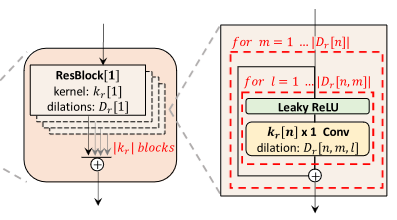
\includegraphics[width=0.8\linewidth]{hifigan-blocks.png}
  \caption{Illustration of the ResBlockV2 and MRFF blocks in the HiFiGAN architecture}
  \label{fig:hifigan-blocks}
\end{figure}

As depicted in Figure~\ref{fig:hifigan-blocks}, the interplay between these classes ensures that the model does not just learn patterns but also grasps the variability inherent in authentic audio signals.

% The figure above is a placeholder, and you should replace 'hifigan_blocks.png' with the actual image illustrating the ResBlockV2 and MultiReceptiveFieldFusion blocks.


\section{The Generative Component of HiFiGAN}

Central to the HiFiGAN vocoder is the generative network, termed the HiFiGenerator, which is adept at synthesizing high-fidelity waveforms from mel spectrograms.

\subsection{Initialization of the \texttt{HiFiGenerator}}

In the heart of HiFiGAN's generator lies a carefully orchestrated initialization scheme aiming to establish a foundation that is conducive to high-quality audio generation:

\begin{itemize}
  \item \textbf{Convolutional Preprocessing:} The input mel spectrogram first encounters a preprocessing convolutional layer (\verb|conv_pre|), designed to increase the channel dimensionality to prepare for the subsequent upsampling stages.
  
  \item \textbf{Upsampling Blocks:} The core of the generator consists of a sequence of convolutional transpose layers (upsamples). These layers incrementally upscale the representations back to the time-domain waveform's resolution.
  
  \item \textbf{Receptive Field Fusion:} Post-upsampling, the signal flows through Multi-Receptive Field Fusion blocks that blend information from various receptive fields.
  
  \item \textbf{Post-Processing to Waveform:} Finally, the \verb|conv_post| layer caps the generator, reducing the channels to one and applying a hyperbolic tangent activation to shape the waveform properly.
\end{itemize}

Each layer and block within the generator is initialized with weights designed to foster stable gradient flow and convergence from the outset of training.

\subsection{Forward Pass Dynamics}

The forward pass of the HiFiGenerator incarnates the essence of generative modeling by executing the following sequence of operations:

\begin{enumerate}
  \item \textbf{Initial Convolution:} The mel spectrogram enters the realm of the generator and is swiftly projected into a higher-dimensional space.
  
  \item \textbf{Upsample and Fuse:} In a tandem yet orchestrated fashion, the model employs upsampling and multi-receptive field fusion techniques to enrichen the processed audio signal iteratively.
  
  \item \textbf{Final Convolution:} As the culmination of the transformational symphony, the fine-tuned representation is converted into a raw audio waveform by the post-processing convolutional layer.
\end{enumerate}

These sequential transformations enable the HiFiGenerator to breathe life into mere numerical representations, much like a maestro conducting an ensemble to produce symphonies from silence.

\subsection{Conclusion}

The HiFiGenerator functions as a sophisticated, generative powerhouse within the HiFiGAN vocoder, aptly showcasing the model's convolutional elegance and its capability to synthesize audio waveforms with remarkable quality.

\begin{figure}[ht]
  \centering
  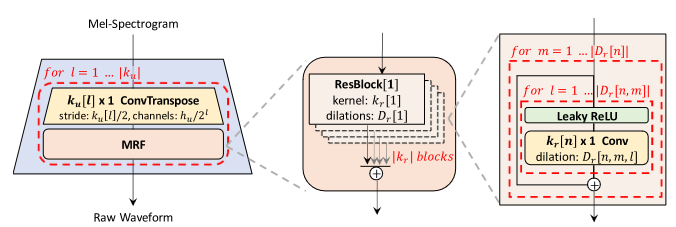
\includegraphics[width=\linewidth]{hifigan-generator.png}
  \caption{Diagram of the waveform generation process in the HiFiGenerator class}
  \label{fig:hifi_generator}
\end{figure}

With the assistance of meticulously chosen hyperparameters and a thoughtful convergence of architectural elements, the HiFiGenerator stands as a testament to modern audio synthesis technology. Its role is paramount, its function elemental, and its output nothing short of extraordinary.

% The figure above is a placeholder. Ensure to update 'hifi_generator.png' with the actual illustration of the generative model.


\section{Discriminative Components of HiFiGAN}

A crucial aspect of the HiFiGAN vocoder is its discriminative network, which captures and exploits the nuanced patterns within audio waveforms. This network consists of a series of discriminators, among them the HiFiDiscriminatorP and HiFiDiscriminatorMultiPeriod classes.

\subsection{The \texttt{HiFiDiscriminatorP} Class}

\begin{itemize}
  
  \item \textbf{Design Philosophy:} The HiFiDiscriminatorP or Period Discriminator operates on the convolutional principle, inspecting audio signals with a critical eye towards periodic textures—akin to seeking rhythm in music.
  
  \item \textbf{Architecture:} It contains a chain of 2D convolutional layers with leaky ReLU activations, each designed to scrutinize the signal at varying resolutions and scales. 
  
  \item \textbf{Specialized Convolution:} In an innovative twist, these layers are designed to operate across different periods of the wave, giving the model a unique insight into the periodic nature of sounds.
  
  \item \textbf{Forward Pass:} When running input data through the network, the tensor is momentarily reshaped to introduce a new dimension -- a clever way to distribute the period across the batch for thorough inspection. Post that, it resumes a more traditional path through the convolutional layers.
  
\end{itemize}

\subsection{The \texttt{HiFiDiscriminatorMultiPeriod} Class}

\begin{itemize}
  
  \item \textbf{Multi-Period Design:} The HiFiDiscriminatorMultiPeriod class takes the innovative concept of period-based discrimination to a new level by combining several HiFiDiscriminatorP instances, each tailored to a unique period, thus capturing a diverse spectrum of acoustic resonances.
  
  \item \textbf{Configurability:} With periods ranging from short (2) to longer (11), it is thoughtfully designed to cover a broader aspect of periodic representations within the audio.
  
  \item \textbf{Composite Features:} The composite output consists of a melding pot of features—each discriminator's view merged into a rich representation of the input data's rhythmic structure.

\end{itemize}

\subsection{Implications for Audio Fidelity}

The inclusion of these discriminators in the network architecture personifies the GAN's adversarial nature. Each brings a critical perspective to the generative process, ensuring that the synthesized audio does not deviate from what is perceptually authentic and true to human hearing.

\begin{figure}[ht]
  \centering
  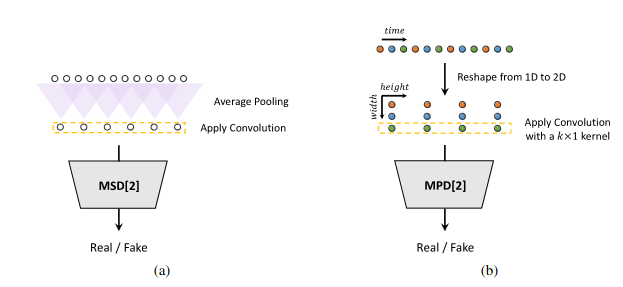
\includegraphics[width=\linewidth]{hifigan-discriminators.png}
  \caption{Schematic of the discriminating process in the Discriminators}
  \label{fig:hifigan-discriminators}
\end{figure}

These discriminators form a rigorous test of the generator's output, serving as a relentless jury that demands authenticity, richness, and fineness in the synthesized sound.

% As usual, remember to replace 'hifigan_discriminators.png' with an actual image file that depicts the described discriminator architectures.


\section{Advancing Fidelity with Scale Discriminators}

The HiFiGAN framework employs a dual-discriminator setup to ensure the comprehensive authenticity of synthesized audio. The second discriminator in this setup is the HiFiDiscriminatorS or Scale Discriminator, paired with its ensemble variant, the HiFiDiscriminatorMultiScale.

\subsection{The \texttt{HiFiDiscriminatorS} Class}

\begin{itemize}
  \item \textbf{Operational Mechanism:} The HiFiDiscriminatorS focuses on evaluating the audio signal through a series of 1D convolutions—each layer designed to focus on different frequency bands and temporal resolutions of the signal.
  
  \item \textbf{Convolution Hierarchy:} It encompasses a cascade of convolutional layers with varying kernel sizes, strides, and groupings, intending to dissect the input signal with increasing granularity.
  
  \item \textbf{Normalization and Activation:} Each convolutional layer is followed by a leaky ReLU activation, introducing non-linearity into the network's decision-making while being normalized through spectral or weight norms to stabilize the training process.
\end{itemize}

\subsection{The \texttt{HiFiDiscriminatorMultiScale} Class}

\begin{itemize}
  \item \textbf{Conceptual Foundation:} The Multi-Scale Discriminator encapsulates a set of HiFiDiscriminatorS instances, each operating at a different scale or resolution to capture a wide array of signal distortions and intricacies.
  
  \item \textbf{Scale-Specific Arbitration:} This ensemble setup amplifies the model's ability to discern details across multiple scales, potentially catching discrepancies invisible to a single scale discriminator.
  
  % Uncomment the following if you decide to describe the average pooling layers' role
  %\item \textbf{Integration with Pooling:} While currently omitted, the design allows for average pooling layers to downscale features for each scale-specific discriminator, further empowering the model's multi-resolution critique.
\end{itemize}

\subsection{Synthesis Judgment and Training}

By engaging these two discriminator types in an intricate adversarial dance with the generator, the HiFiGAN setup aims to train a generator so fine-tuned that it can replicate humanly indistinguishable audio textures—an ultimate testament to machine learning's emulation prowess.

\begin{figure}[ht]
  \centering
  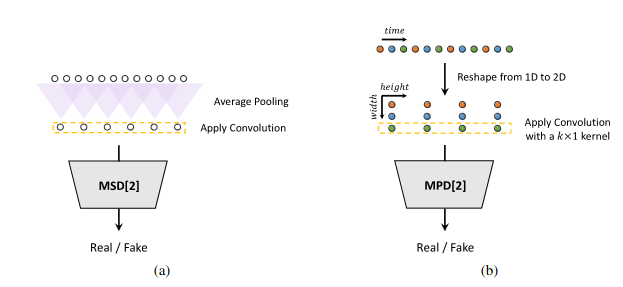
\includegraphics[width=\linewidth]{hifigan-discriminators.png}
  \caption{The operational flow within the Scale and Multi-Scale Discriminators}
  \label{fig:hifigan-discriminators}
\end{figure}

The Scale Discriminators are critical to the High-Fidelity target of HiFiGAN, enforcing a rigorous auditing of the generative output across various auditory facets of detail and quality.

% Replace 'hifigan_scales_discriminators.png' with the actual visual representation file of the Scale and Multi-Scale Discriminators.


\section{Harmonizing Synthesis with HiFiGAN}

The HiFiGAN class encapsulates the full generative adversarial network, harmonizing the generator with not one, but two discriminators, in a symphony of neural computations that birth audio outputs of stunning quality.

\subsection{The Unified \texttt{HiFiGAN} Class}

The HiFiGAN serves as the conductor of this sophisticated ensemble, cueing each component at the precise moment to play its part in the audio generation process.

\begin{itemize}
  \item \textbf{The Generator:} At the core sits the HiFiGenerator, an artist wielding neural networks to paint waveforms from spectral canvases of mel spectrograms faithfully.
  
  \item \textbf{Dual Discriminators:} Complementing the generator are two sets of ears—the HiFiDiscriminatorMultiPeriod and HiFiDiscriminatorMultiScale, each with a keen sense for the nuances of audio. They critique the generator's compositions, pushing for ever-closer approximations of the real deal.
  
  \item \textbf{Loss Calculation Within Forward Pass:} In a rather innovative twist, the HiFiGAN forward pass doesn't just propagate signals; it also judges them, computing the loss in tandem—and thereby fully encapsulating the learning process.
\end{itemize}

\subsection{Operational Workflow}

\begin{enumerate}
  \item \textbf{Audio Generation:} The class begins its act by instructing the HiFiGenerator to transform mel spectrograms into preliminary audio.
  
  \item \textbf{Discriminator Evaluation:} The dual discriminators then take the stage, assessing both the real and generated audio to provide feedback. Ingeniously, their evaluation differs depending on whether they focus on generator improvements or discriminator finesse.
  
  \item \textbf{Loss Integration:} Finally, the discriminators' feedback culminates in a loss function, which becomes the compass guiding future performances towards more convincing territory.
\end{enumerate}

\subsection{Inference Mode}

In a separate act, the inference mode, the network foregoes the adversarial critique, focusing solely on rendering the generator’s creative prowess into audible content from an input mel spectrogram.

%\begin{figure}[ht]
%  \centering
%  \includegraphics[width=\linewidth]{hifigan_full_model.png}
%  \caption{Architectural overview of the HiFiGAN showing the generator and discriminator interactions}
%  \label{fig:hifigan_full_model}
%\end{figure}

Conclusively, HiFiGAN epitomizes the essence of generative adversarial networks—learning not through isolated toil but through a vibrant interplay of creation and criticism, a paradigm that yields audio not just synthesized, but virtually alive.

% Ensure to update 'hifigan_full_model.png' with the actual visual representation of the complete HiFiGAN model, showing the interactions between the generator and discriminators.


\section{The Art of Learning: Loss Computation in HiFiGAN}

In the training symphony of HiFiGAN, loss functions play first violin, conducting the adjustment of weights with decisive strokes. Let's delve into these functions, the mathematical muse behind the network's learning.

\subsection{Feature Matching Loss}

\begin{itemize}
  \item \textbf{Harmonizing Features:} The \verb|features_loss| function orchestrates a harmony between the features extracted from the real and synthesized audio by the discriminators, quantifying the difference using the mean absolute error. 

  \item \textbf{Intuitive Interpretation:} Each layer of discriminator output contributes to the symphony of features, and the function ensures that the fake outputs closely mirror the composition of the real ones, note by note.
\end{itemize}

\subsection{Generator Loss}

The generator's performance is evaluated by \verb|the generator_loss| function:

\begin{itemize}
  \item \textbf{The Critique of Discordance:} This function frames the generator's ultimate goal to create output indistinguishable from reality in the ear of the discriminators.
  
  \item \textbf{Choreography for Deception:} The discriminators' output serves as a measure of verisimilitude, with the loss encouraging the generator's output to be mistaken by the discriminators for the real deal.
  
  \item \textbf{Compositional Nuance:} By striving to push the discriminator outputs towards one, the generator is artistically tuning its outputs to the key of authenticity.
\end{itemize}

\subsection{Discriminator Loss}

\begin{itemize}
  \item \textbf{Dual Perspectives in Criticism:} \verb|discriminator_loss| evaluates the discriminators' ability to differentiate between the real and fake, rewarding discernment and penalizing confusion.
  
  \item \textbf{The Duality of Loss:} Seeking an equilibrium, the loss is computed separately for genuine and artificial inputs, then summed up to coax the discriminators towards a balance of skepticism and belief.
\end{itemize}

\subsection{Mel-Spectrogram Loss}

Finally, the fidelity of the audio synthesis to the original mel spectrogram is kept in check by \verb|mel_loss|:

\begin{itemize}
  \item \textbf{Anchoring the Tune:} This loss ensures that the generator stays true to the 'sheet music'—the mel spectrogram—by penalizing deviations from the given melodic structure.
  
  \item \textbf{Keeping the Tempo:} The L1 norm—the difference between each pitch in the predicted and target spectrograms—maintains the generator's tempo, ensuring it composes audio that not only sounds right but follows the right score.
\end{itemize}

\subsection{Conducting the Learning Orchestra}

Each loss component plays a critical role in steering the network towards generating waveforms that are not just realistic but also true to the given melodic conditioning. Like a maestro directing a grand musical performance, these losses together shape the learning trajectory of the HiFiGAN towards the highest echelons of audio synthesis.

\begin{figure}[ht]
  \centering
  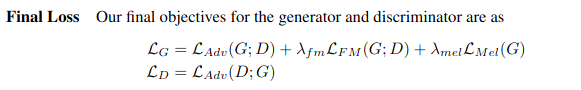
\includegraphics[width=\linewidth]{hifigan-loss-functions.png}
  \caption{A representation of the total loss functions guiding the HiFiGAN's training concert}
  \label{fig:hifigan-loss-functions}
\end{figure}

With the baton of these loss functions, the network diligently refines its parameters, learning to strike the perfect pitch and tempo to echo the original performance.

% Remember to substitute 'hifigan_loss_functions.png' with the actual graphic that illustrates the loss functions in the algorithm's operation.


ection{The Crescendo of Learning: Total Loss Calculation in HiFiGAN}

Calculating the total loss in HiFiGAN represents the crescendo in the model's training, harmonizing all the loss components to fine-tune its generative abilities.

\subsection*{The Composition of Total Loss}

\begin{itemize}
  \item \textbf{Adversarial Loss:}
  \begin{itemize}
    \item The generator's adversarial performance is critiqued twice, once for each discriminator, through the \verb|loss_gen1| and \verb|loss_gen2|. This encourages the generator to craft audio indistinguishable from the real by both scales of judgment.
    
    \item In parallel, \verb|loss_disc1| and \verb|loss_disc2| measure each discriminator's success at accurately detecting real versus fake, refining their discerning ears.
  \end{itemize}
  
  \item \textbf{Feature Matching Loss:}
  \begin{itemize}
    \item Feature matching loss is the harmony between the real and fake feature outputs from each discriminator, encapsulated in \verb|loss_fm1| and \verb|loss_fm2|. Doubling this loss accentuates its importance in the model's priority.
  \end{itemize}
  
  \item \textbf{Mel-Spectrogram Loss:}
  \begin{itemize}
    \item Ensuring fidelity to the original mel-spectrogram, \verb|loss_mel| penalizes any dissonance between the input and generated melodic structures.
    \item This loss is amplified 45 times, emphasizing the model's attention to accurately recreate the melodic contours.
  \end{itemize}
\end{itemize}

\subsection*{Symphonic Summary}

Combining these losses yields \verb|loss_total|, striking a balance between generative creativity and discriminative precision. The ret dictionary not only holds the overall loss but also itemizes each component, documenting the detailed nuances of the network's performance, akin to a setlist of a symphonic performance.

\subsection*{Monitoring Mean Discriminator Outputs}

Additionally, the model computes the mean response of each discriminator for both real and fake audio. These insights (\verb|mean_disc1_on_real|, \verb|mean_disc1_on_fake|, etc.) are like audience applause, a real-time feedback for the network's conductor to adjust the ensemble's output in subsequent iterations.

\subsection*{The HiFiGAN Training Performance}

With the total loss as its guide, HiFiGAN polishes each note in the generative process. The interplay between the loss components shapes the adversarial training, each iteration bringing the network closer to the virtuoso ability to generate audio of exquisite realism and fidelity.

\begin{figure}[ht]
  \centering
  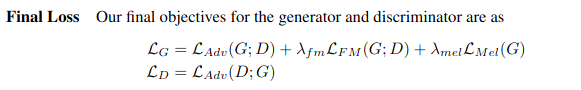
\includegraphics[width=\linewidth]{hifigan-loss-functions.png}
  \caption{Illustration of the total loss computation and its components within the HiFiGAN training cycle.}
  \label{fig:hifigan-loss-functions}
\end{figure}

The model is an opus where the losses are not simply errors but rather the notes that compose the harmony of learning, leading to a glorious crescendo of simulated sound, indistinguishable from the real audio spectrum.

% Remember to replace 'hifigan_total_loss.png' with the actual visualization representing the total loss calculation process inside HiFiGAN.


\section{Data Collation for Deep Learning: \texttt{nv\_collate\_fn}\\ and \texttt{get\_collate\_fn}}

In any machine learning pipeline, preparing the data for the model is as crucial as the model's architecture itself. For batch processing, data collation functions are the unsung heroes, ensuring that each dataset item fits perfectly into the training batch with the elegance of a puzzle piece finding its right place. We will focus on two such functions tailored for specific datasets in the context of automated speech recognition (ASR) and neural vocoding (NV).

\subsection{\texttt{nv\_collate\_fn}}

\begin{itemize}
  \item \textbf{The Dynamics of Padding:} The function \texttt{nv\_collate\_fn} assembles a batch from dataset items by padding the tensors to match the longest sequence within the batch. This ensures uniformity, allowing for seamless parallel computations on the batch.

  \item \textbf{Efficient Memory Allocation:} To avoid memory wastage, only the necessary padding is added to each sequence to reach the maximum length in the batch, not a byte more.

  \item \textbf{Length Tracking:} It catalogues the original lengths of the sequences before padding, facilitating operations that may require this information downstream in the pipeline, like masking out the padding in loss computations.
\end{itemize}

\subsection{\texttt{get\_collate\_fn}}

\begin{itemize}
  \item \textbf{Dataset-Specific Logic:} This dispatcher function, \texttt{get\_collate\_fn}, serves as a switchboard, linking each dataset with its respective collate function based on the dataset type, ensuring that each one gets the tailored treatment it requires.
  
  \item \textbf{Adaptive Handling:} For instance, LibrispeechDataset would be paired with an ASR-specific collate function, while LJSpeechDataset or VocoderTestDataset would utilize the NV-specific \texttt{nv\_collate\_fn} outlined above.
\end{itemize}

\subsection{Ensuring Smooth Data Flow}

Together, these two functions exemplify the meticulous backstage work of a deep learning system, working diligently to ensure that the spotlighted model can perform without a hitch, singing arias or synthesizing speech with the same ease.

%\begin{figure}[ht]
%  \centering
%  \includegraphics[width=\linewidth]{data_collation_flowchart.png}
%  \caption{Flowchart demonstrating the selection and execution process of data collation functions based on dataset types.}
%  \label{fig:data_collation_flowchart}
%\end{figure}

In essence, \texttt{nv\_collate\_fn} and \texttt{get\_collate\_fn} are much akin to the stagehands of a theatrical production, working behind the curtains to set the stage for the performers—the data—to shine in the limelight of the model's computational theatre.

% Replace 'data_collation_flowchart.png' with an actual image that depicts how the get_collate_fn function selects the appropriate collation function based on the dataset type.


\section{The \texttt{NVTrainer} Class: Conducting the Neural Vocoder Training}

\subsection{Initialization and Configuration}

The \texttt{NVTrainer}, an articulate class inherited from \texttt{BaseTrainer}, sets the stage for the training process of neural vocoders. Adapting to the varied cadences of epoch-based or iteration-based training, this class finely tunes the orchestration of data flow, learning rate adjustments, and the calculated cadence of logging and metric tracking.

\subsubsection{Configurable Parameters}

Within its constructor, it presents a comprehensive suite of parameters:
\begin{itemize}
  \item \texttt{model}: The neural network model to be trained.
  \item \texttt{metrics}: Criteria for assessing performance.
  \item \texttt{optimizer}: The algorithm that adjusts model weights.
  \item \texttt{config}: A configuration dictionary to manage settings.
  \item \texttt{device}: The hardware destination for tensor computation.
  \item \texttt{dataloaders}: A dictionary housing training and evaluation loaders.
  \item \texttt{lr\_scheduler}: An optional argument for learning rate modification.
  \item \texttt{len\_epoch}: Defines the length of an epoch based on dataset size.
  \item \texttt{skip\_oom}: A flag to bypass out-of-memory errors during training.
\end{itemize}

\subsubsection{Metric Management}

The class tracks metrics meticulously:
\begin{itemize}
  \item A layered \texttt{MetricTracker} object holds the progressive learning stages, combining traditional metrics with those bespoke to neural vocoders—like generator and discriminator losses.
  \item Additionally, it upholds a vigilant watch over gradient norms, ensuring the stability of the learning process.
\end{itemize}

\subsubsection{Batch and Device Management}

A static method \texttt{move\_batch\_to\_device} diligently ensures that each element of the training batch is transferred to the device at hand, be it GPU or otherwise, for efficient operations.

\subsection{Gradual Refinements}

\texttt{NVTrainer} emphasizes the importance of maintaining the integrity of the gradient's magnitude through \texttt{\_clip\_grad\_norm}, an internal method that leverages configuration settings to clip gradients and prevent the infamous exploding gradient problem.

\subsection{\texttt{\_train\_epoch} Method}

The class equips itself with the \texttt{\_train\_epoch} method as it ventures to encapsulate the intricacies of a training epoch, marking the core steps where the bulk of learning takes place.

\subsection{Closing Note}

With the \texttt{NVTrainer} class, a neural vocoder's training becomes a symphony, each parameter and method a note in a grand composition that produces the harmonious flow of learning and model improvement over time.

%\begin{figure}[ht]
%  \centering
%  \includegraphics[width=\linewidth]{nvtrainer_overview.png}
%  \caption{Graphical overview of the NVTrainer class highlighting key functionalities and data flow.}
%  \label{fig:nvtrainer_overview}
%\end{figure}

% Make sure to replace 'nvtrainer_overview.png' with an actual image that diagrams the NVTrainer class, encapsulating its structure and functionalities.


\subsection{The \texttt{\_train\_epoch} Method: A Training Epoch in Action}

The \texttt{\_train\_epoch} method is the heart of the training process, where each epoch unfurls through meticulous iteration over data batches. This method not only drives the learning through forward and backward passes but echoes each step with insightful metric tracking and robust logging, ensuring each epoch's performance is faithfully recorded.

\begin{enumerate}
  \item \textbf{Commence Training}: The model enters training mode, and metrics are reset for a fresh start.
  \item \textbf{Data Iteration}: Each data batch from the loader is processed with a display of progress thanks to \texttt{tqdm}.
  \item \textbf{Batch Processing}: The batch is sent to \texttt{process\_batch}, thoroughly prepared and primed for training iteration.
  \item \textbf{Memory Management}: Encountering out-of-memory errors triggers a graceful skip, releasing gradient memory and clearing cache if so configured by the \texttt{skip\_oom} flag.
  \item \textbf{Metric Tracking}: Gradient norms are diligently updated in the tracker after each batch.
  \item \textbf{Logging Intervals}: At specific intervals, detailed logs are recorded, including scalar values for loss and learning rates, and visual logs for predictions and spectrograms.
  \item \textbf{Evaluation}: If an evaluation dataloader is provided, the method concludes an epoch with a validation step, often including additional metrics and loss measurements. 
\end{enumerate}

Every batch and epoch concludes with a symphonic compilation of metrics—like a musical score, the output is a complex layering of notes (metrics) coming together to describe the performance of the training at that moment.


\subsection{Eloquent Epoch Execution}

With precision and clarity, the \texttt{\_train\_epoch} method manifests the iterative training process, capturing the essence of learning over iterations with a steadfast rhythm of computations and evaluations, all while being guarded by meticulous metric monitoring and logging.

\subsection{Visualization and Audio Logging}

Calling into action the chosen metrics and learning artifacts, the method records the synthesized and original audio and mel-spectrograms, offering an auditory account of the model’s progress. Each spectrogram and audio snippet is a note in the wider melody of the model's development.

\subsection{Concluding with the Transcription of Learning}

As the epoch draws to a close, the assembled statistics and insights form a comprehensive log—a testament to the knowledge accrued within the epoch's span, ready to be conveyed back into the flow of training epochs and further refinement.

%\begin{figure}[ht]
%  \centering
%  \includegraphics[width=\linewidth]{training_epoch_flow.png}
%  \caption{Flowchart of the \texttt{\_train\_epoch} method, capturing the symphony of operations throughout a training epoch in the NVTrainer class.}
%  \label{fig:training_epoch_flow}
%\end{figure}

% Replace 'training_epoch_flow.png' with a genuine diagram detailing the flow of operations within a training epoch as guided by the \texttt{\_train\_epoch} method.


\subsection{Method Details of \texttt{NVTrainer}}

Taking a closer look at the two pivotal methods of the \texttt{NVTrainer} class:\ \texttt{process\_batch} and \texttt{\_evaluation\_epoch}. Let's frame each method like a scene in a screenplay, brimming with technical prose.

\subsubsection{\texttt{process\_batch} Method}

The \texttt{process\_batch} method meticulously translates data batches into the language of tensors, moving them onto the device for computation. Each batch is a scene of its own:

\begin{enumerate}
  \item The scenery is set as the batch make its grand entrance by being ushered onto the computational device.
  \item If the curtain is up for training, gradients are wiped clean to make way for the new act.
  \item The model, now in the spotlight, performs its forward pass—interpreting audio and mel to produce losses and outputs.
  \item Should the outputs form a dictionary, the batch is seamlessly expanded.
  \item A switch to the training mode allows the backpropagation, handing the directorial baton to the optimizer to adjust the model’s parameters.
  \item Should a learning rate scheduler be part of the cast, it adjusts the tempo with a step after the optimizer's move.
  \item Finally, the metrics tracker records the ensemble of losses and other performance measures, readying them for the curtain call.
\end{enumerate}

The stage is thus set for learning, with metrics captured for future reference and analysis, preparing the cast for the next scene.


\subsubsection{\texttt{\_evaluation\_epoch} Method}

Meanwhile, \texttt{\_evaluation\_epoch} audits the model’s performance, akin to a dress rehearsal, running through batches without backpropagation:

\begin{enumerate}
  \item The model, in its evaluation attire, freezes parameters for a consistent performance.
  \item As batches parade through the evaluation, they are assessed without the pressure of training, under the watchful eye of metrics that remember each move.
  \item Upon completion of the evaluation dance, the metrics are logged and visual insights of the real and synthesized data are complied into tangible artifacts.
\end{enumerate}

Thus concludes an epoch's validation—the meticulous collection of performance snapshots, capturing the essence of the model's progress.


Both the \texttt{process\_batch} and \texttt{\_evaluation\_epoch} methods form the backbone of the \texttt{NVTrainer}'s methodology, exemplifying a seamless blend of computation, error-checking, performance tracking, and optimization that together define the training and validation journey of a neural vocoder.


\subsection{The Supporting Acts in \texttt{NVTrainer}'s Ensemble}

In every training drama, there are crucial supporting characters—the methods and functions—that ensure the lead performance shines. Here's a look at some of the unsung heroes in \texttt{NVTrainer}.

\subsubsection{The \texttt{\_progress} Method}
The method \texttt{\_progress} serves up a real-time status snapshot:
\begin{enumerate}
  \item Computes the current iteration's progress based on batch index and total samples.
  \item Elegantly prints out the progress as a percentage of completion.
\end{enumerate}
Its charming simplicity betrays its importance in keeping track of training advances—truly, a glance into the rearview mirror during the journey.

\subsubsection{Log Methods: \texttt{\_log\_spectrogram} and \texttt{\_log\_audio}}
With \texttt{\_log\_spectrogram} and \texttt{\_log\_audio}, these methods take snapshots of stories told by data:
\begin{enumerate}
  \item One showcases the spectral landscape—an imaging of sound—via random selection for visual feedback.
  \item The other echoes the auditory data back into the world, letting one hear the model's vocal fruits as it learns to sing the data's tune.
\end{enumerate}
Both employ random sampling, allowing for sporadic yet insightful peeks into the batch's compiled chorus.

\subsubsection{Monitoring the Model's Strait: \texttt{get\_grad\_norm}}
Guarding against the surges in gradient flow is \texttt{get\_grad\_norm}, a vigilant lighthouse:
\begin{enumerate}
  \item It computes the aggregate norm of gradients, a gauge of how fiercely the neural winds are blowing through the network's parameters.
  \item It ensures the network sails smoothly through the tempest of training, uninhibited by the capricious gusts of vanishing or exploding gradients.
\end {enumerate}
Without it, the model's journey might falter in silent numerical storms, unseen but cataclysmic.

\subsubsection{The Chronicler: \texttt{\_log\_scalars}}
\texttt{\_log\_scalars} - A scribe for performance metrics:
\begin{enumerate}
  \item Diligently records the averages of tracked metrics, inscribing them in the annals of tensorboard for posterity.
  \item Ensures no act of learning, no moment of performance improvement, goes unnoticed or unrecorded.
\end{enumerate}
In the nexus of improvement, this method marks the waypoints, keeping track and time of the learning odyssey.

\subsubsection{The Art of Masking: \texttt{mask\_length}}
Lastly, the \texttt{mask\_length} - a refined touch to the data preparation:
\begin{enumerate}
  \item Its purpose is concise: zero out the tensor elements beyond the specified lengths.
  \item It ensures models focus on the melody of data, not the noise, reinforcing the clean harmony intended in each batch.
\end{enumerate}
Think of it as sheet music with rest notes—where silence is as important as the sound.

\subsection{Ensemble in Harmony}
Each method plays its part in the training symphony. Whether illuminating the path ahead, capturing the resonant frequencies, gently guiding the model's learning, or recording its tales of growth, the NVTrainer relies on this ensemble of supporting functionality.


\clearpage

\section{HiFi-GAN Architectural Overview}

\begin{figure}[H]
  \centering
  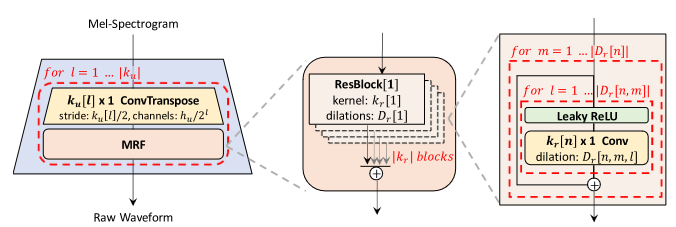
\includegraphics[width=0.6\textwidth]{hifigan-generator.png}
  \caption{HiFi-GAN Generator Architecture}
  \label{fig:hifigan-generator}
\end{figure}

\begin{figure}[H]
  \centering
  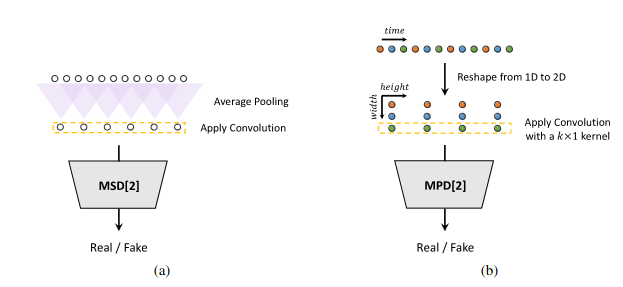
\includegraphics[width=0.6\textwidth]{hifigan-discriminators.png}
  \caption{HiFi-GAN Discriminator Architectures}
  \label{fig:hifigan-discriminators}
\end{figure}

\begin{figure}[H]
  \centering
  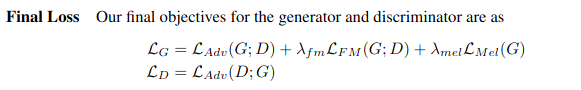
\includegraphics[width=0.6\textwidth]{hifigan-loss-functions.png}
  \caption{HiFi-GAN Loss Function Components}
  \label{fig:hifigan-loss-functions}
\end{figure}


\section{The run before main run}

Before the main run, I have trained the Generator on the mel loss alone to ensure that it works. It worked! In short, mel was 0.3


\section{Training metrics and loss comparisons of the main run}

The duration of that last run was approximately 15 hours. It had 300 epochs, 400 batches per epoch, 16 samples for batch, sequence length 8192 (approximately 370ms with our sample rate 22050Hz)

\begin{figure}[H]
  \centering
  \begin{subfigure}{\textwidth}
    \centering
    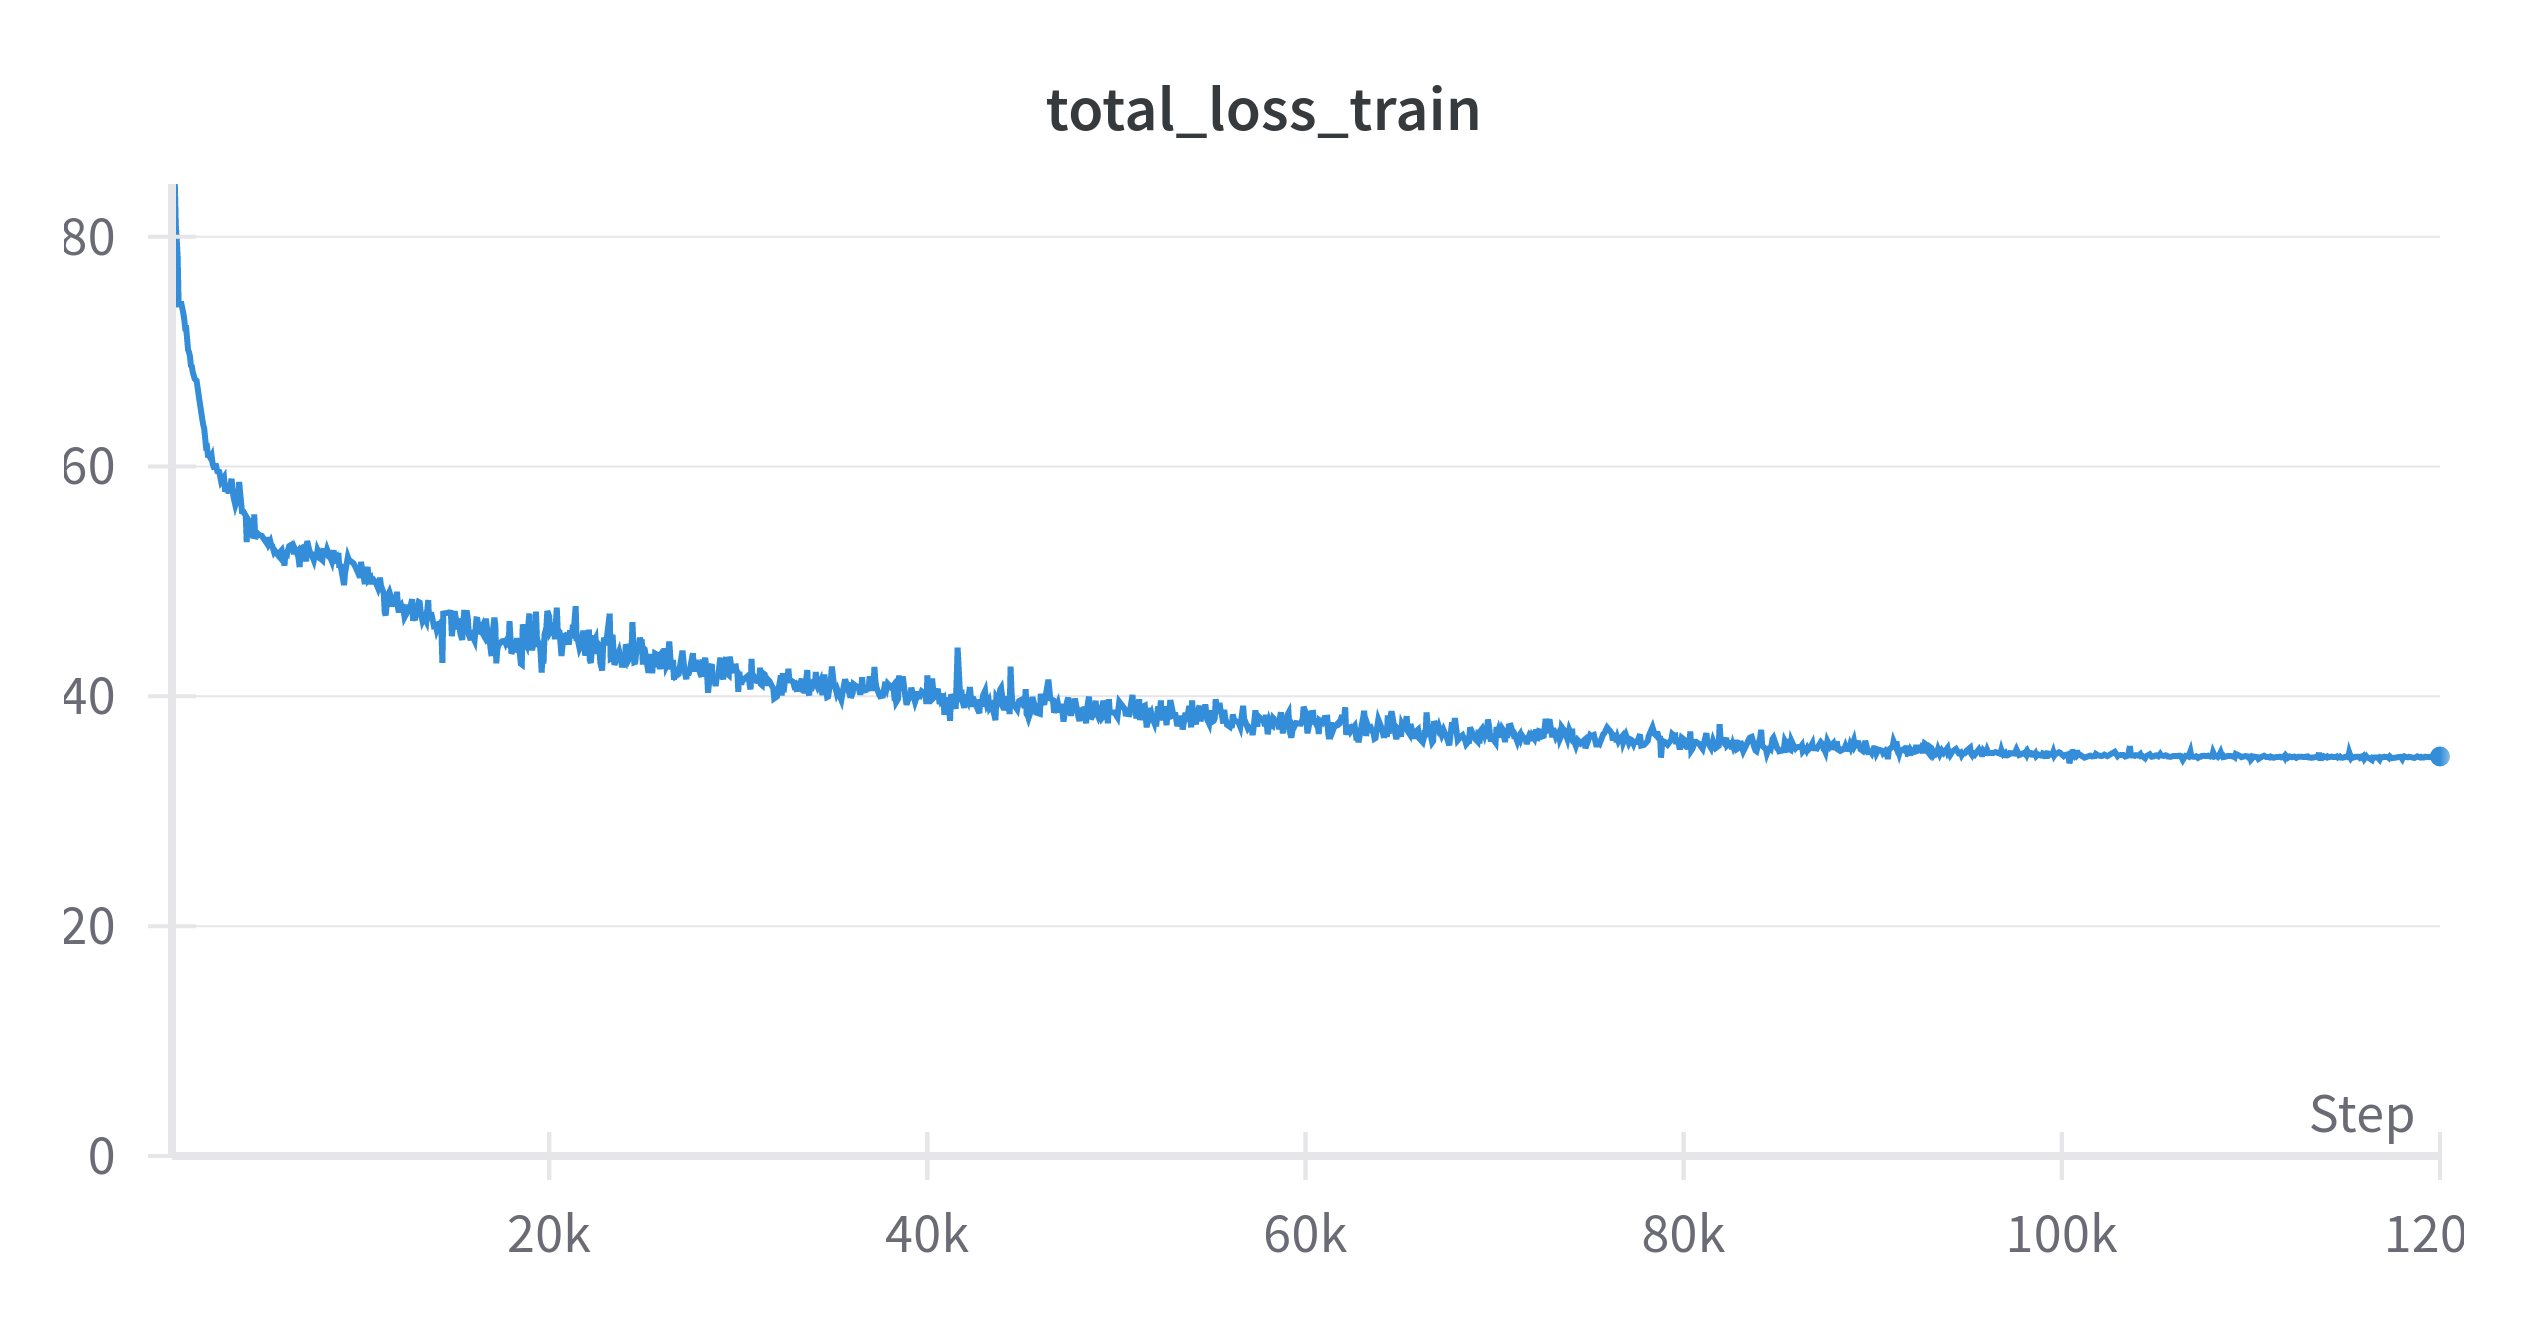
\includegraphics[width=\linewidth]{total-loss-train.png}
    \caption{Total Loss during Training}
    \label{fig:total-loss-train}
  \end{subfigure}
  \hfill
  \begin{subfigure}{\textwidth}
    \centering
    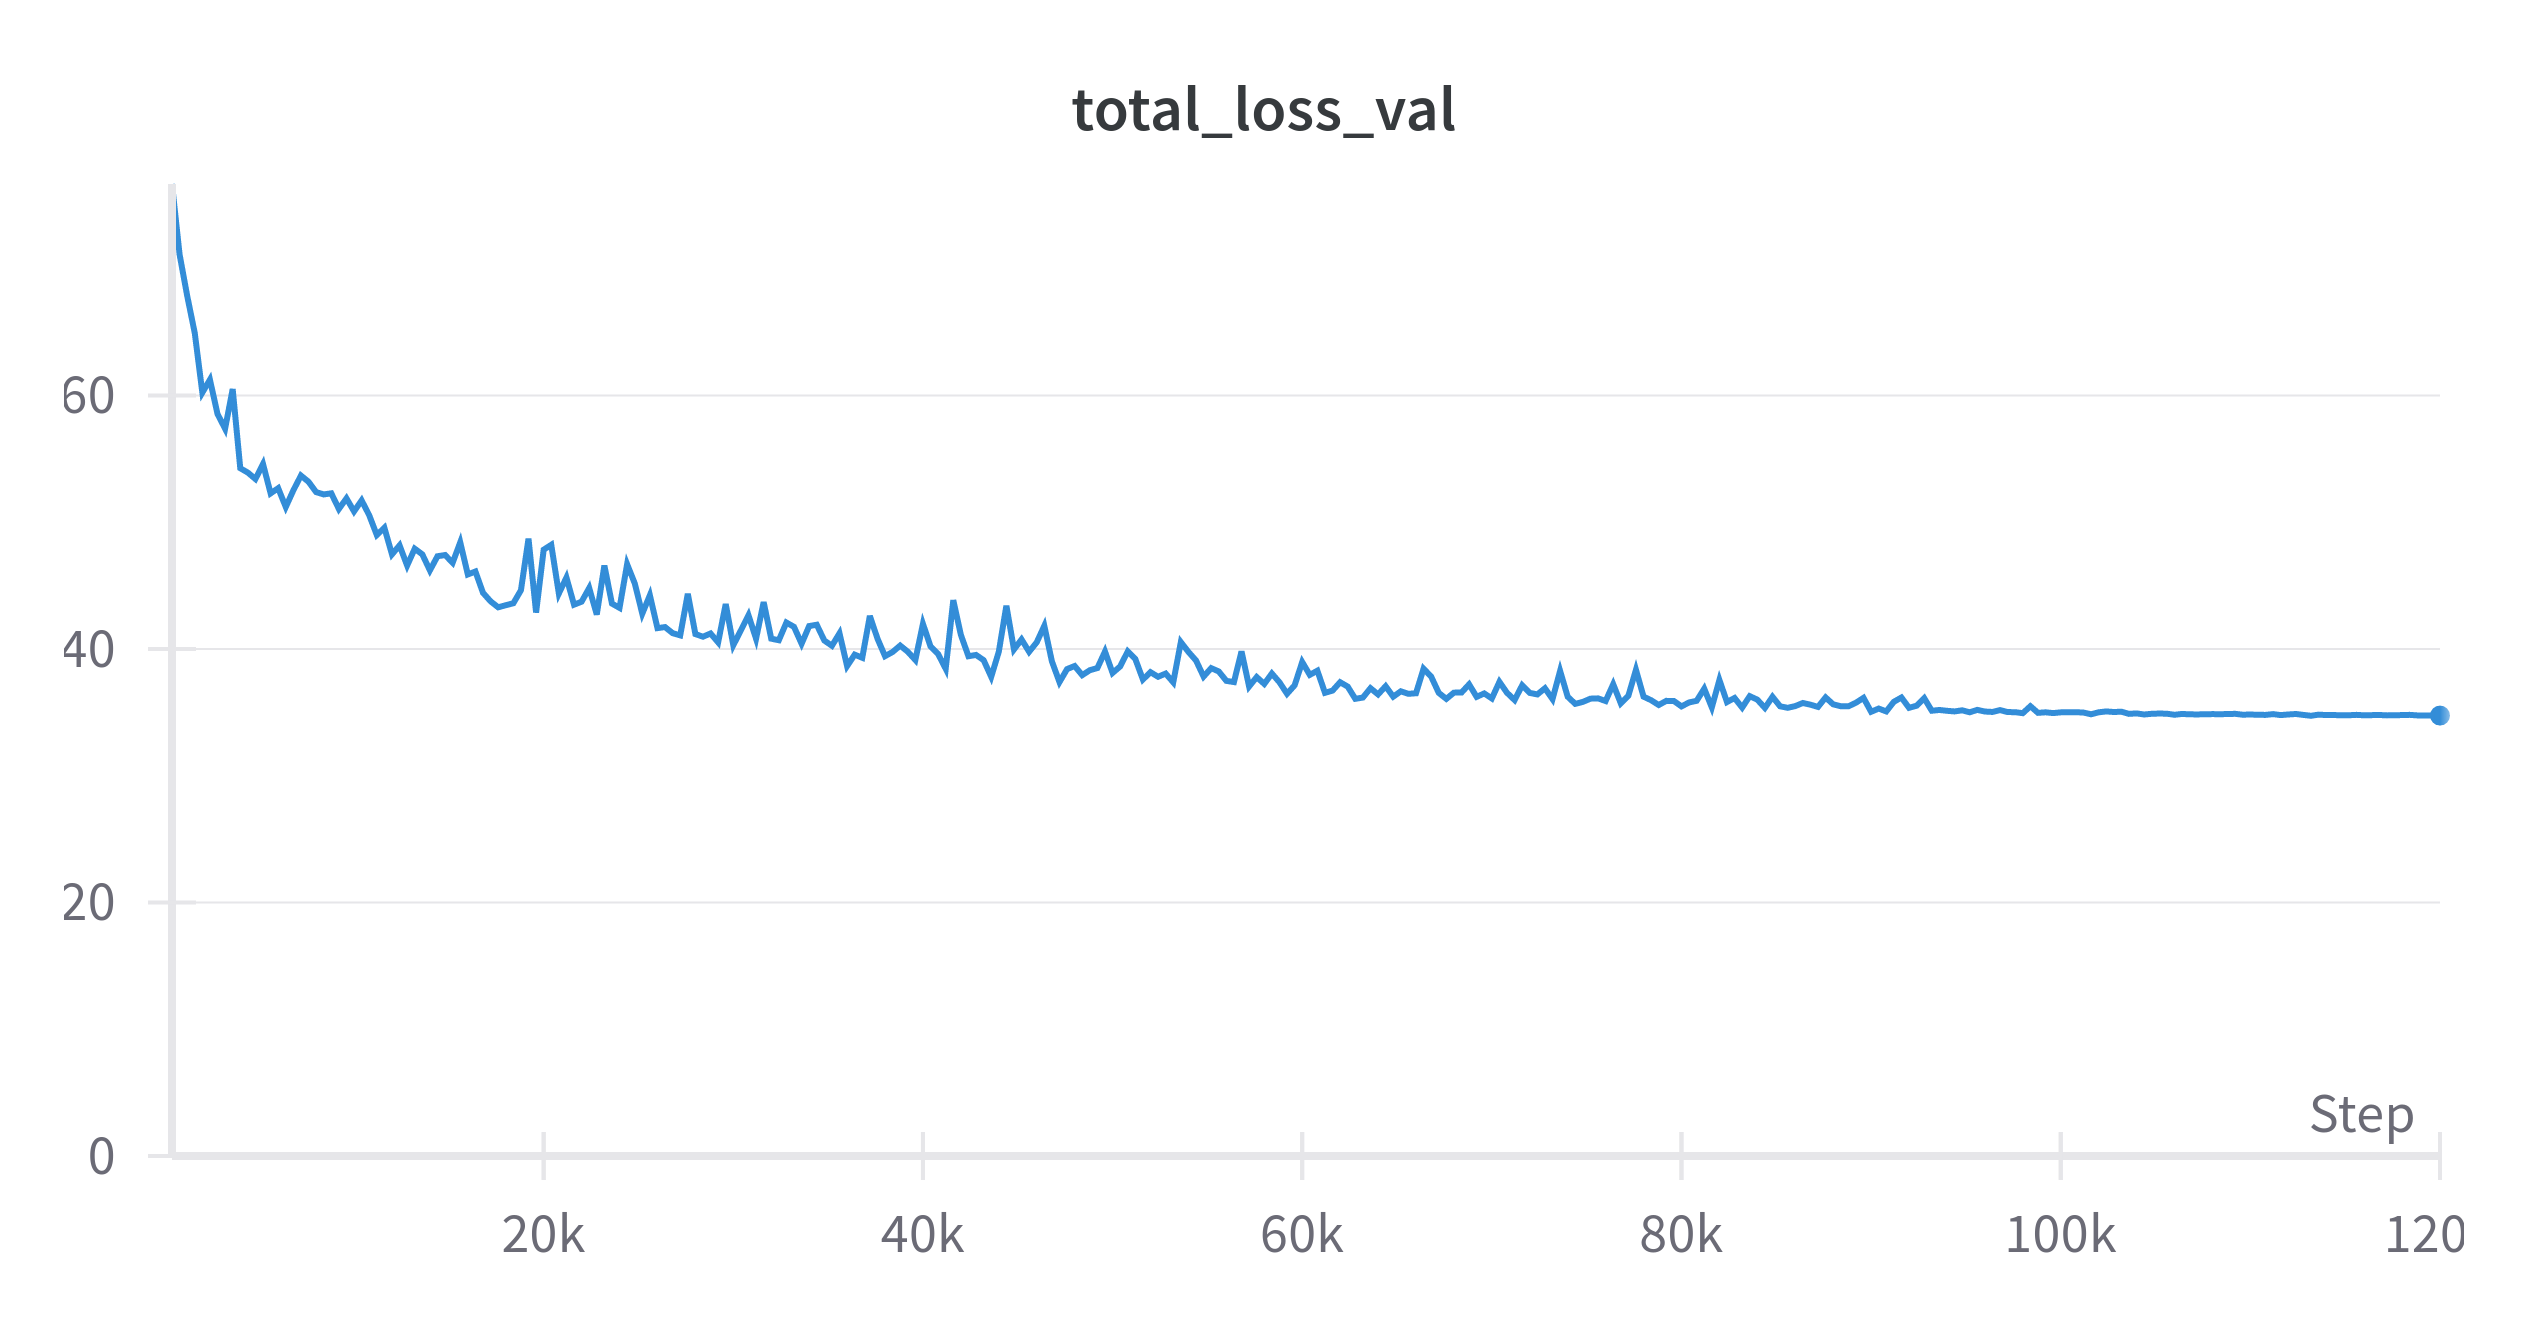
\includegraphics[width=\linewidth]{total-loss-val.png}
    \caption{Total Loss during Validation}
    \label{fig:total-loss-val}
  \end{subfigure}
  \caption{Total Loss comparison between Training and Validation Phases}
\end{figure}

\begin{figure}[H]
  \centering
  \begin{subfigure}{\textwidth}
    \centering
    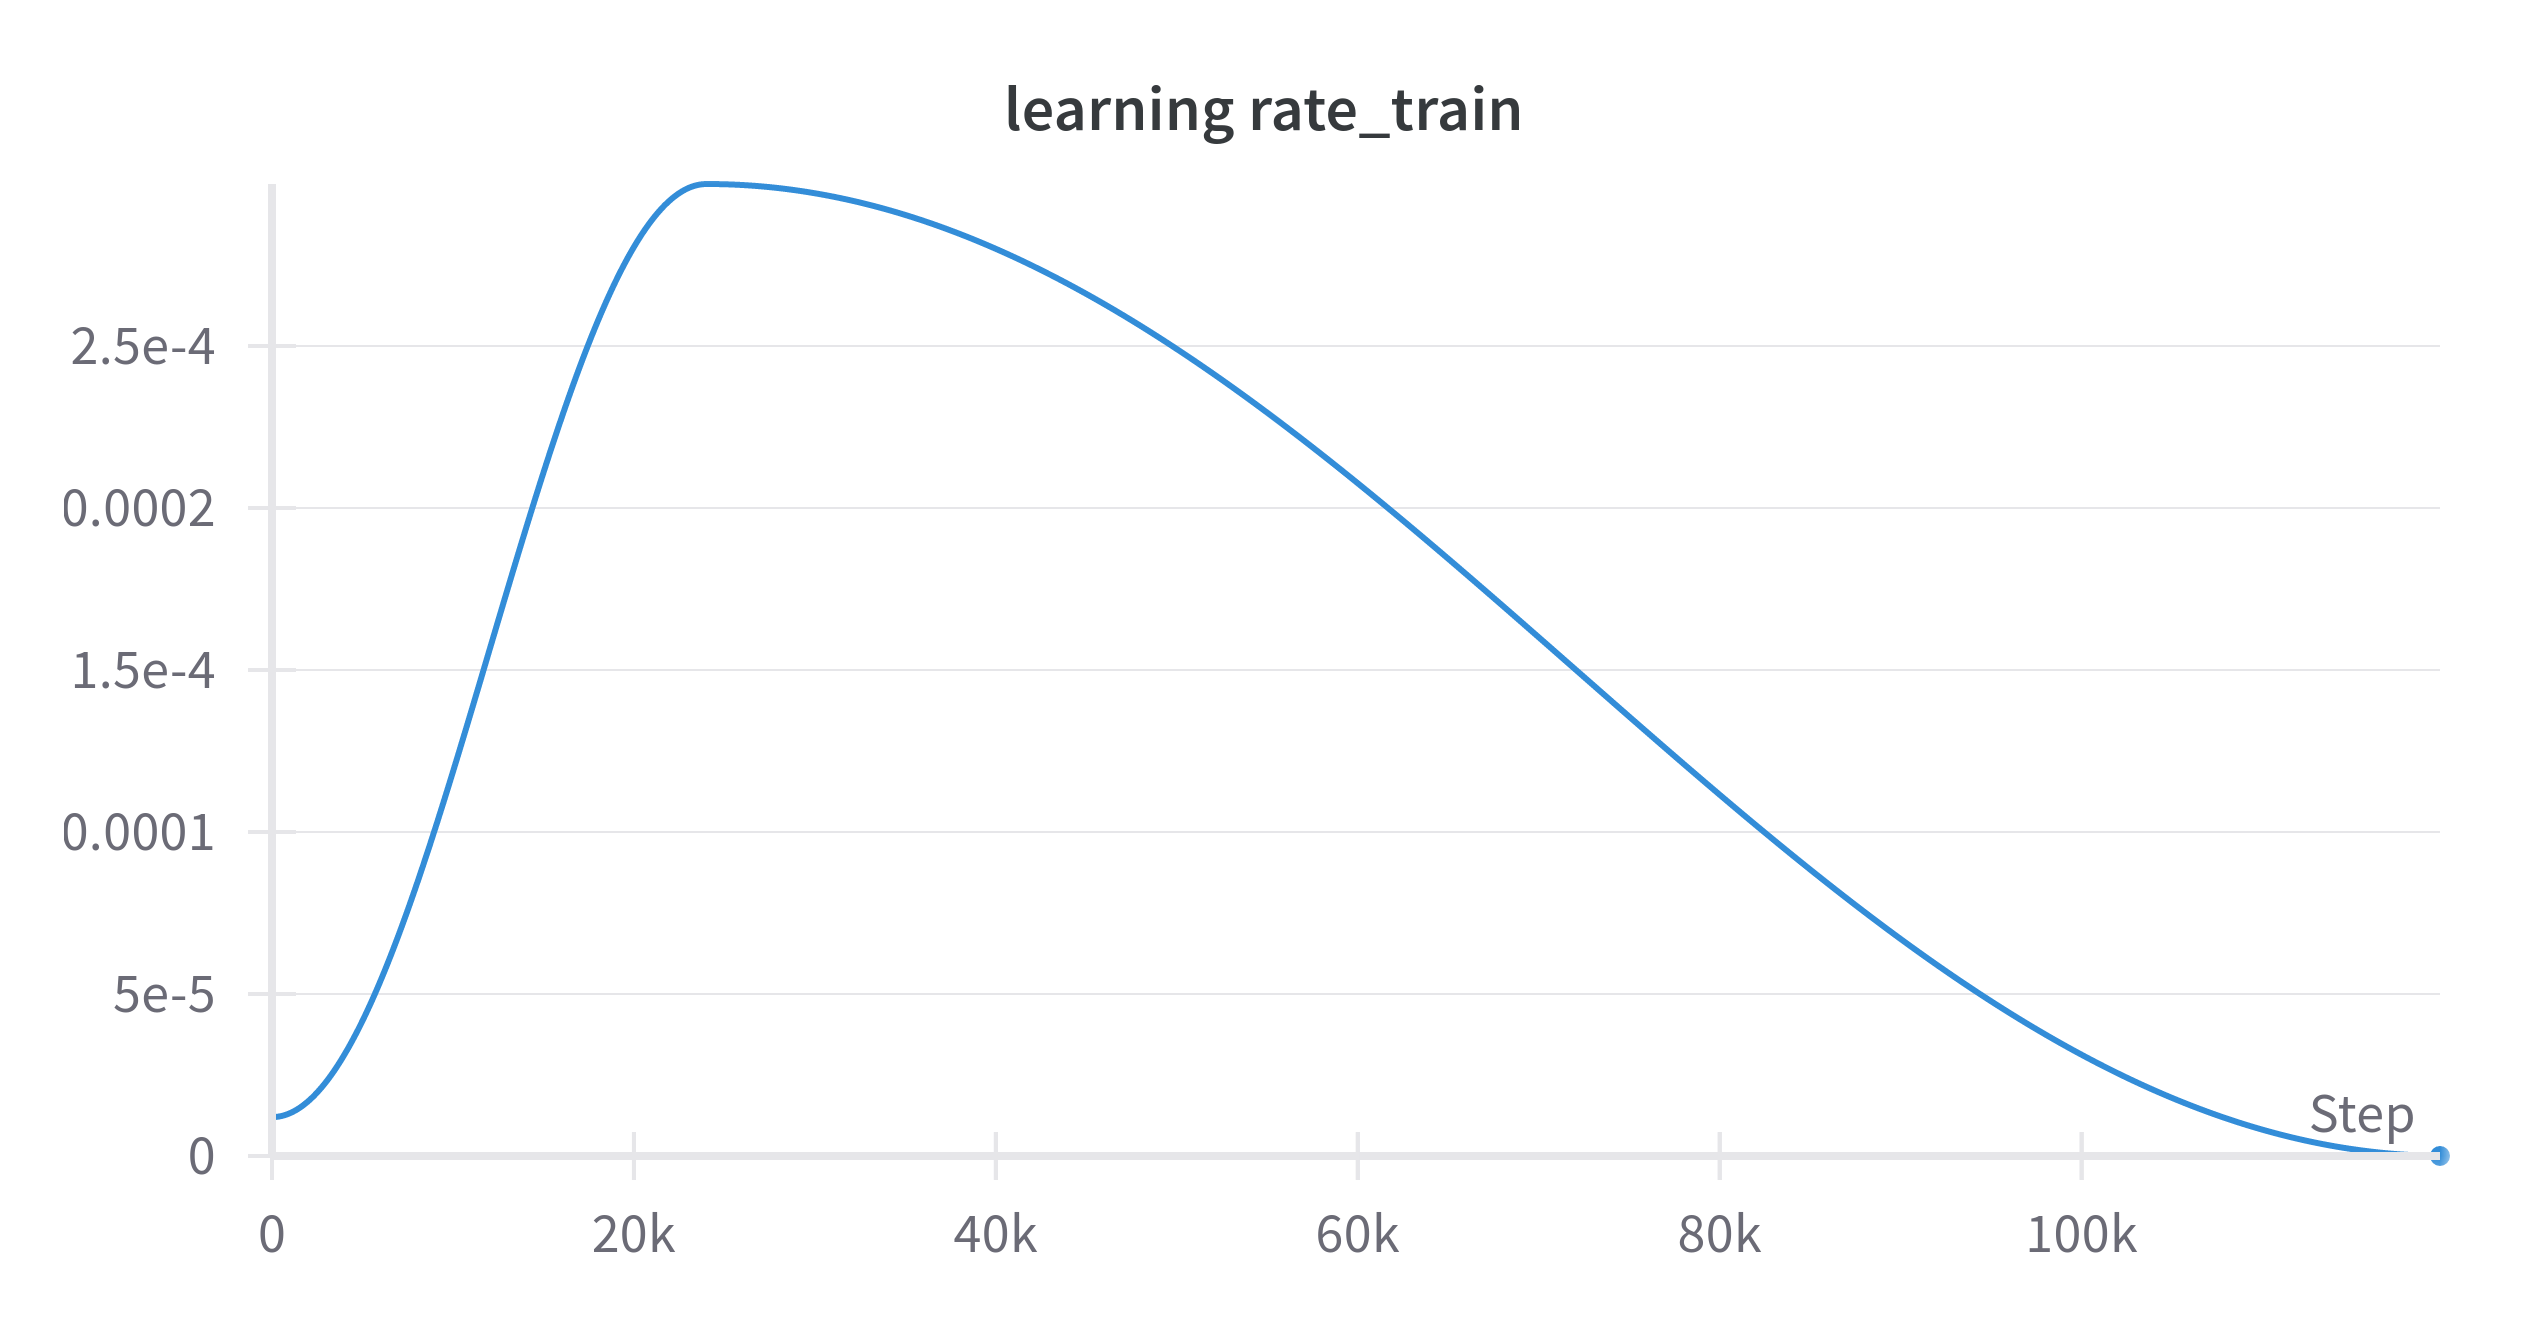
\includegraphics[width=\linewidth]{learning-rate-train.png}
    \caption{Learning Rate over Training}
    \label{fig:learning-rate-train}
  \end{subfigure}%
  \hfill
  [...] % Repeat this pattern for each pair of training/validation loss
  \caption{Various Training and Validation Loss Comparisons}
\end{figure}

% Table for direct comparison, assuming these are smaller, less important plots
\begin{table}[H]
  \centering
  \begin{tabular}{ccc}
    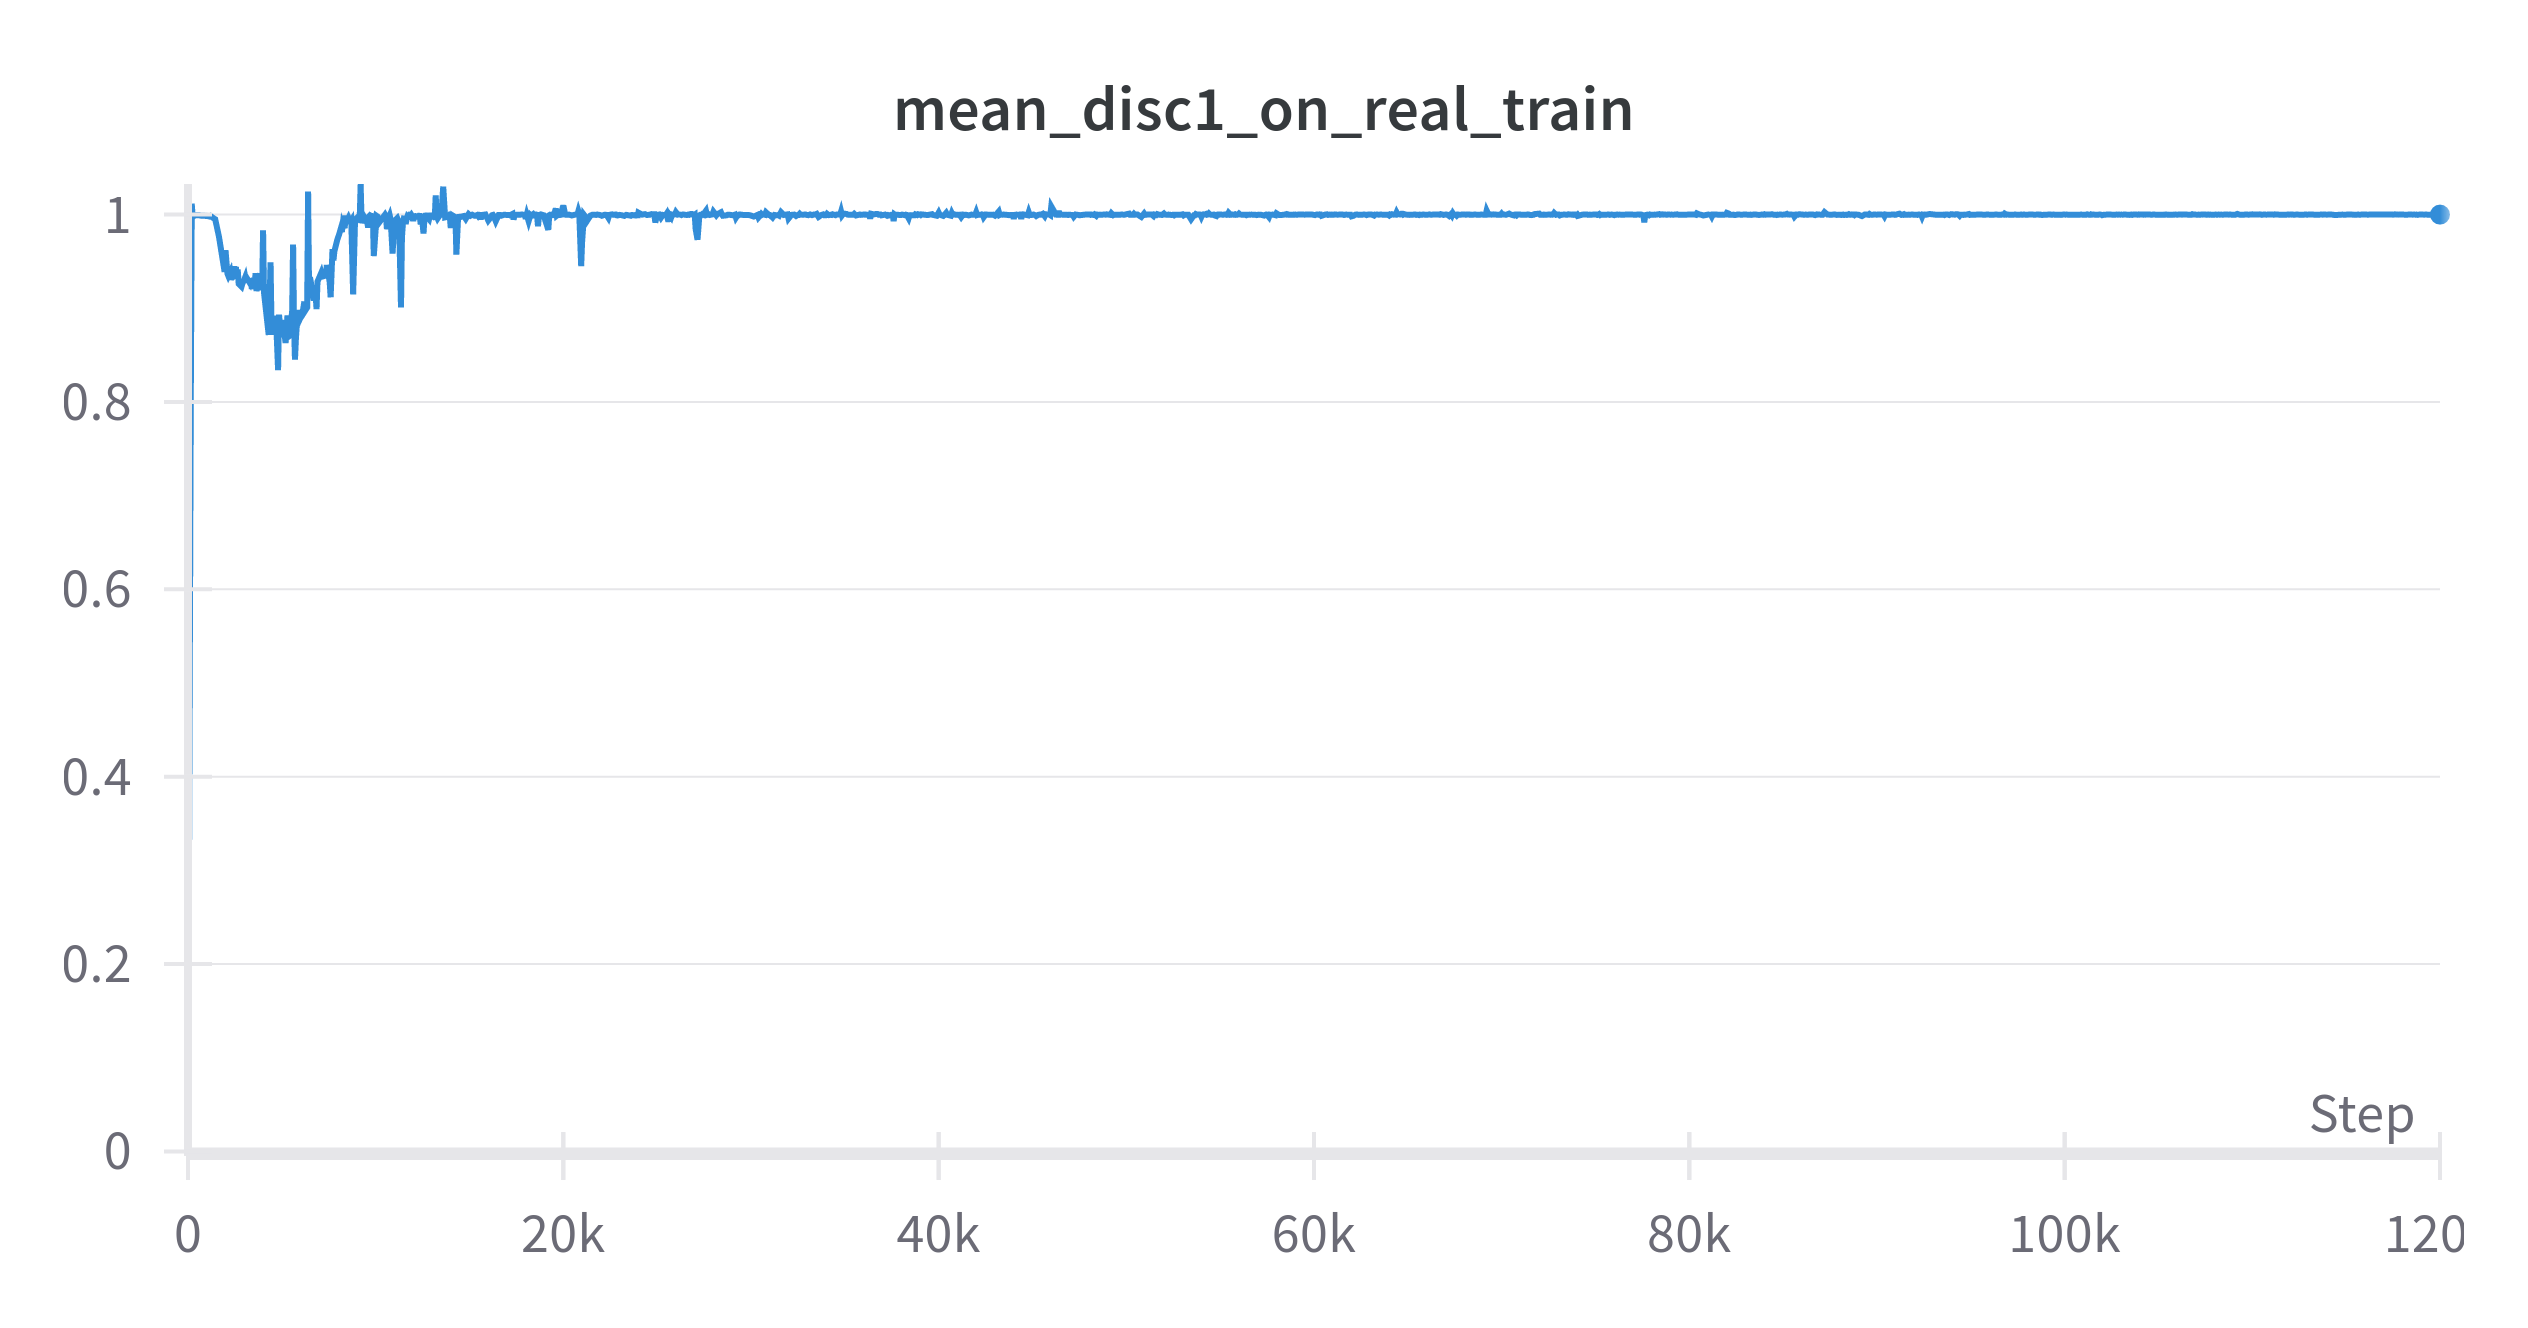
\includegraphics[width=0.4\textwidth]{mean-disc1-on-real-train.png} &
    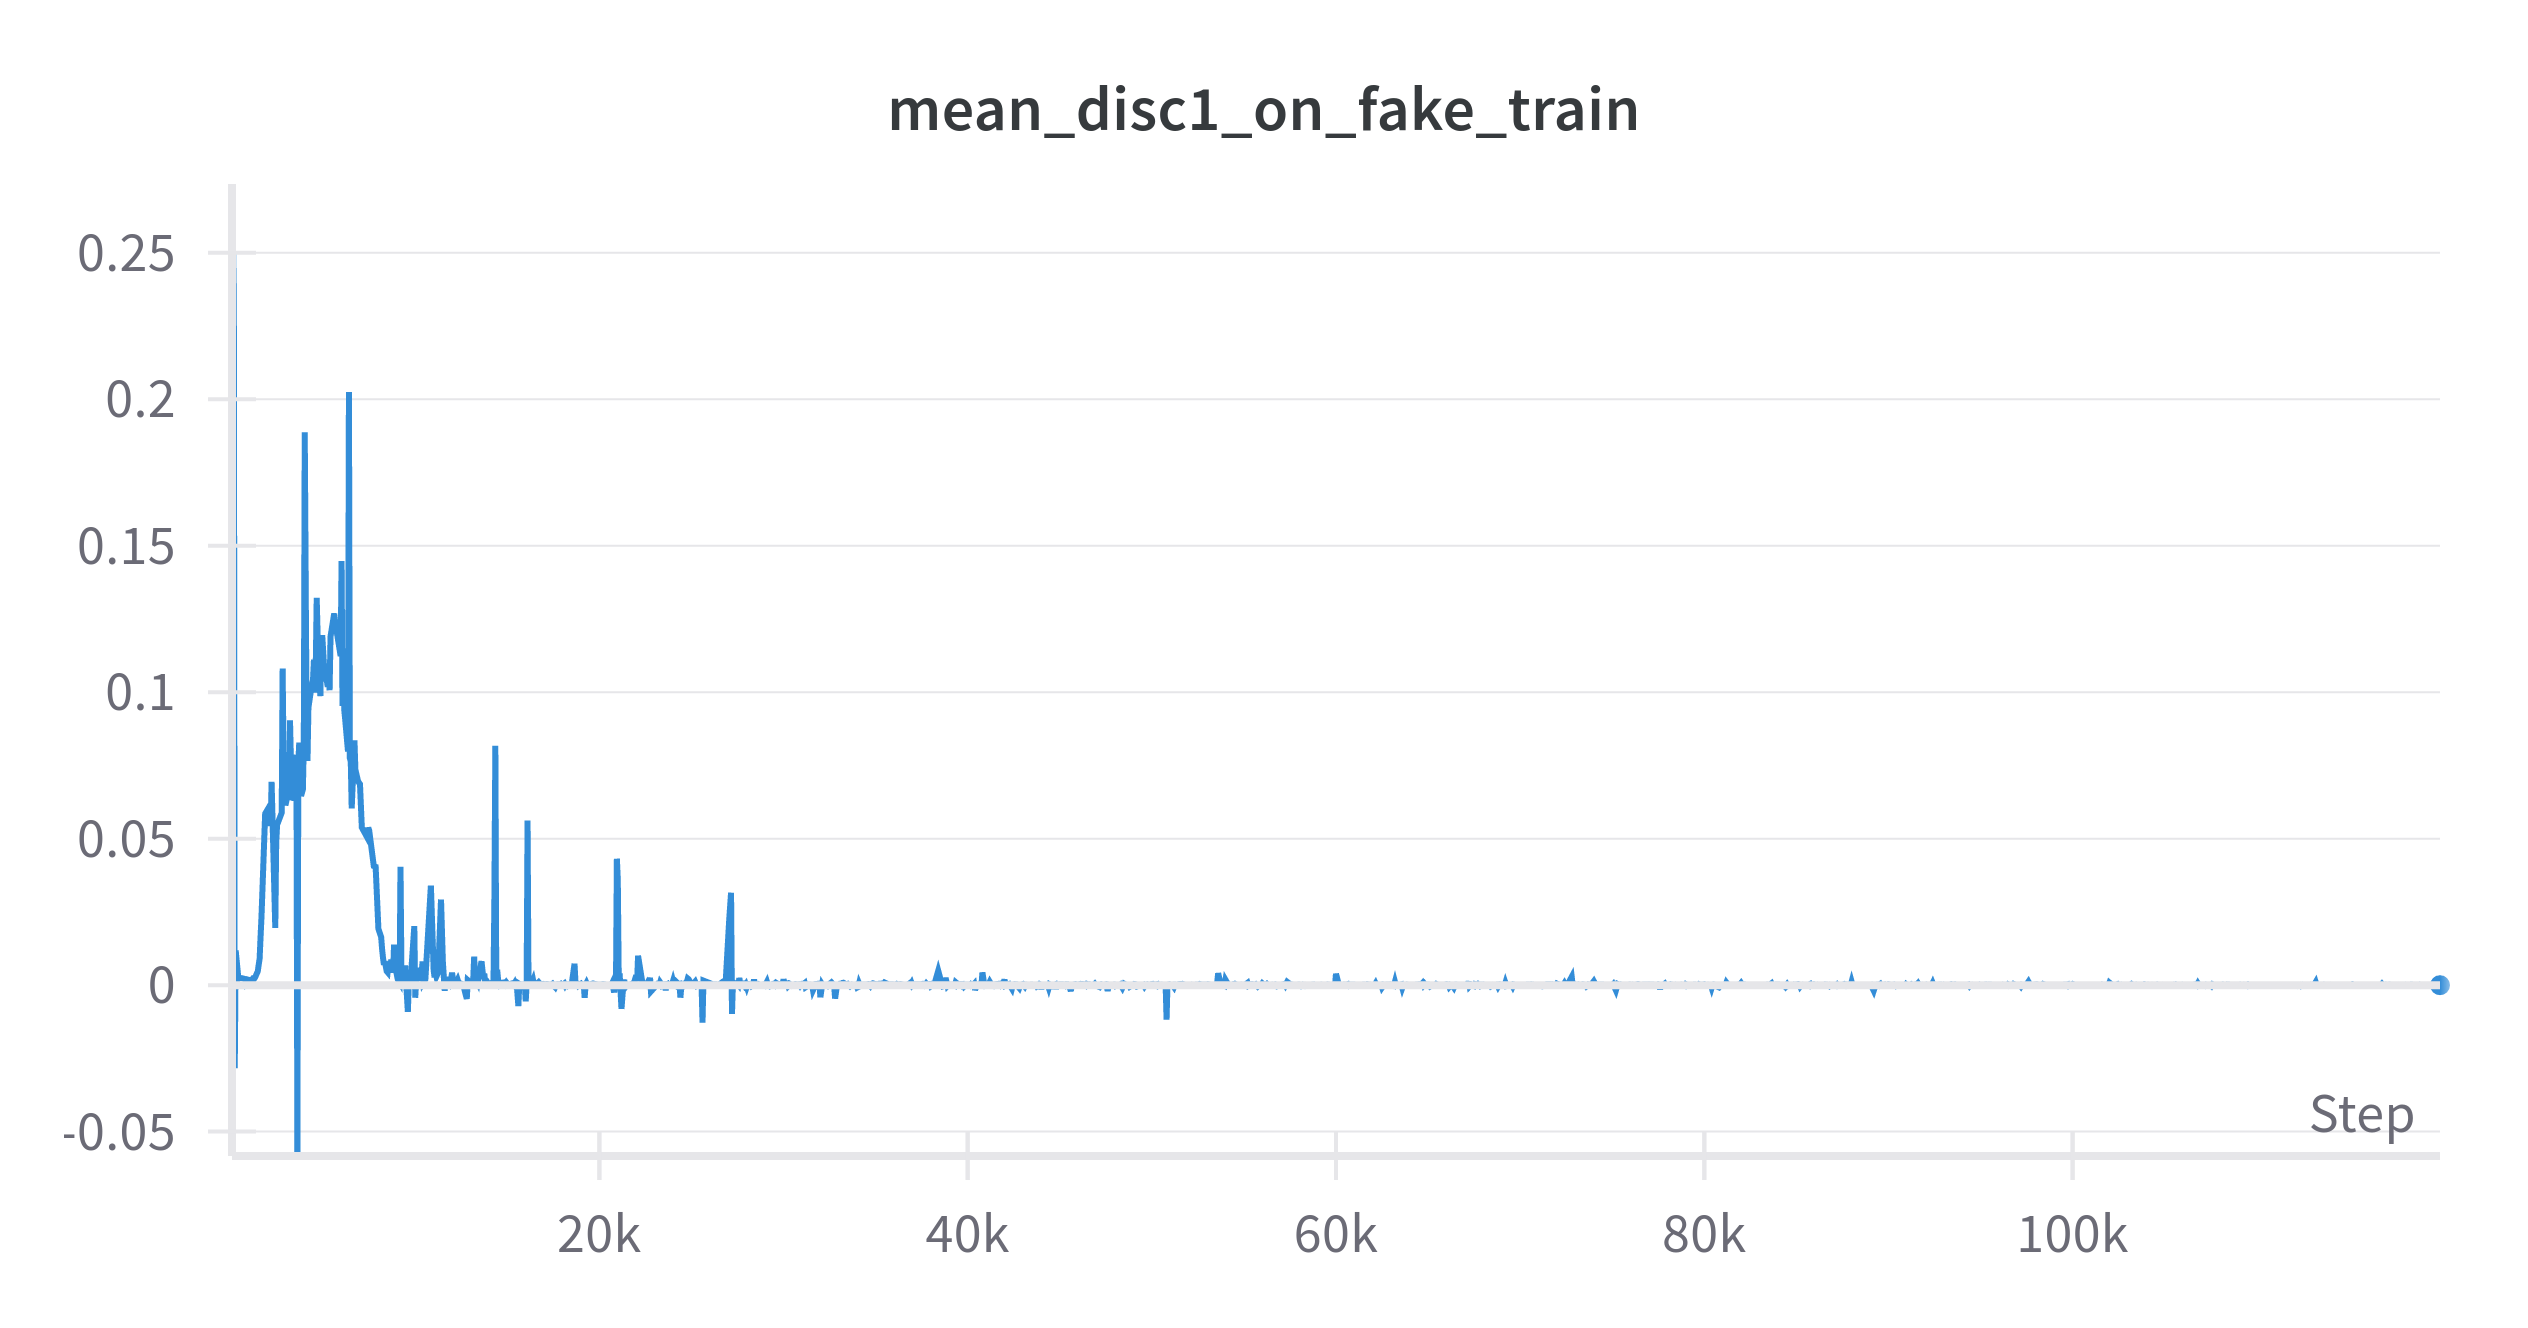
\includegraphics[width=0.4\textwidth]{mean-disc1-on-fake-train.png} &
    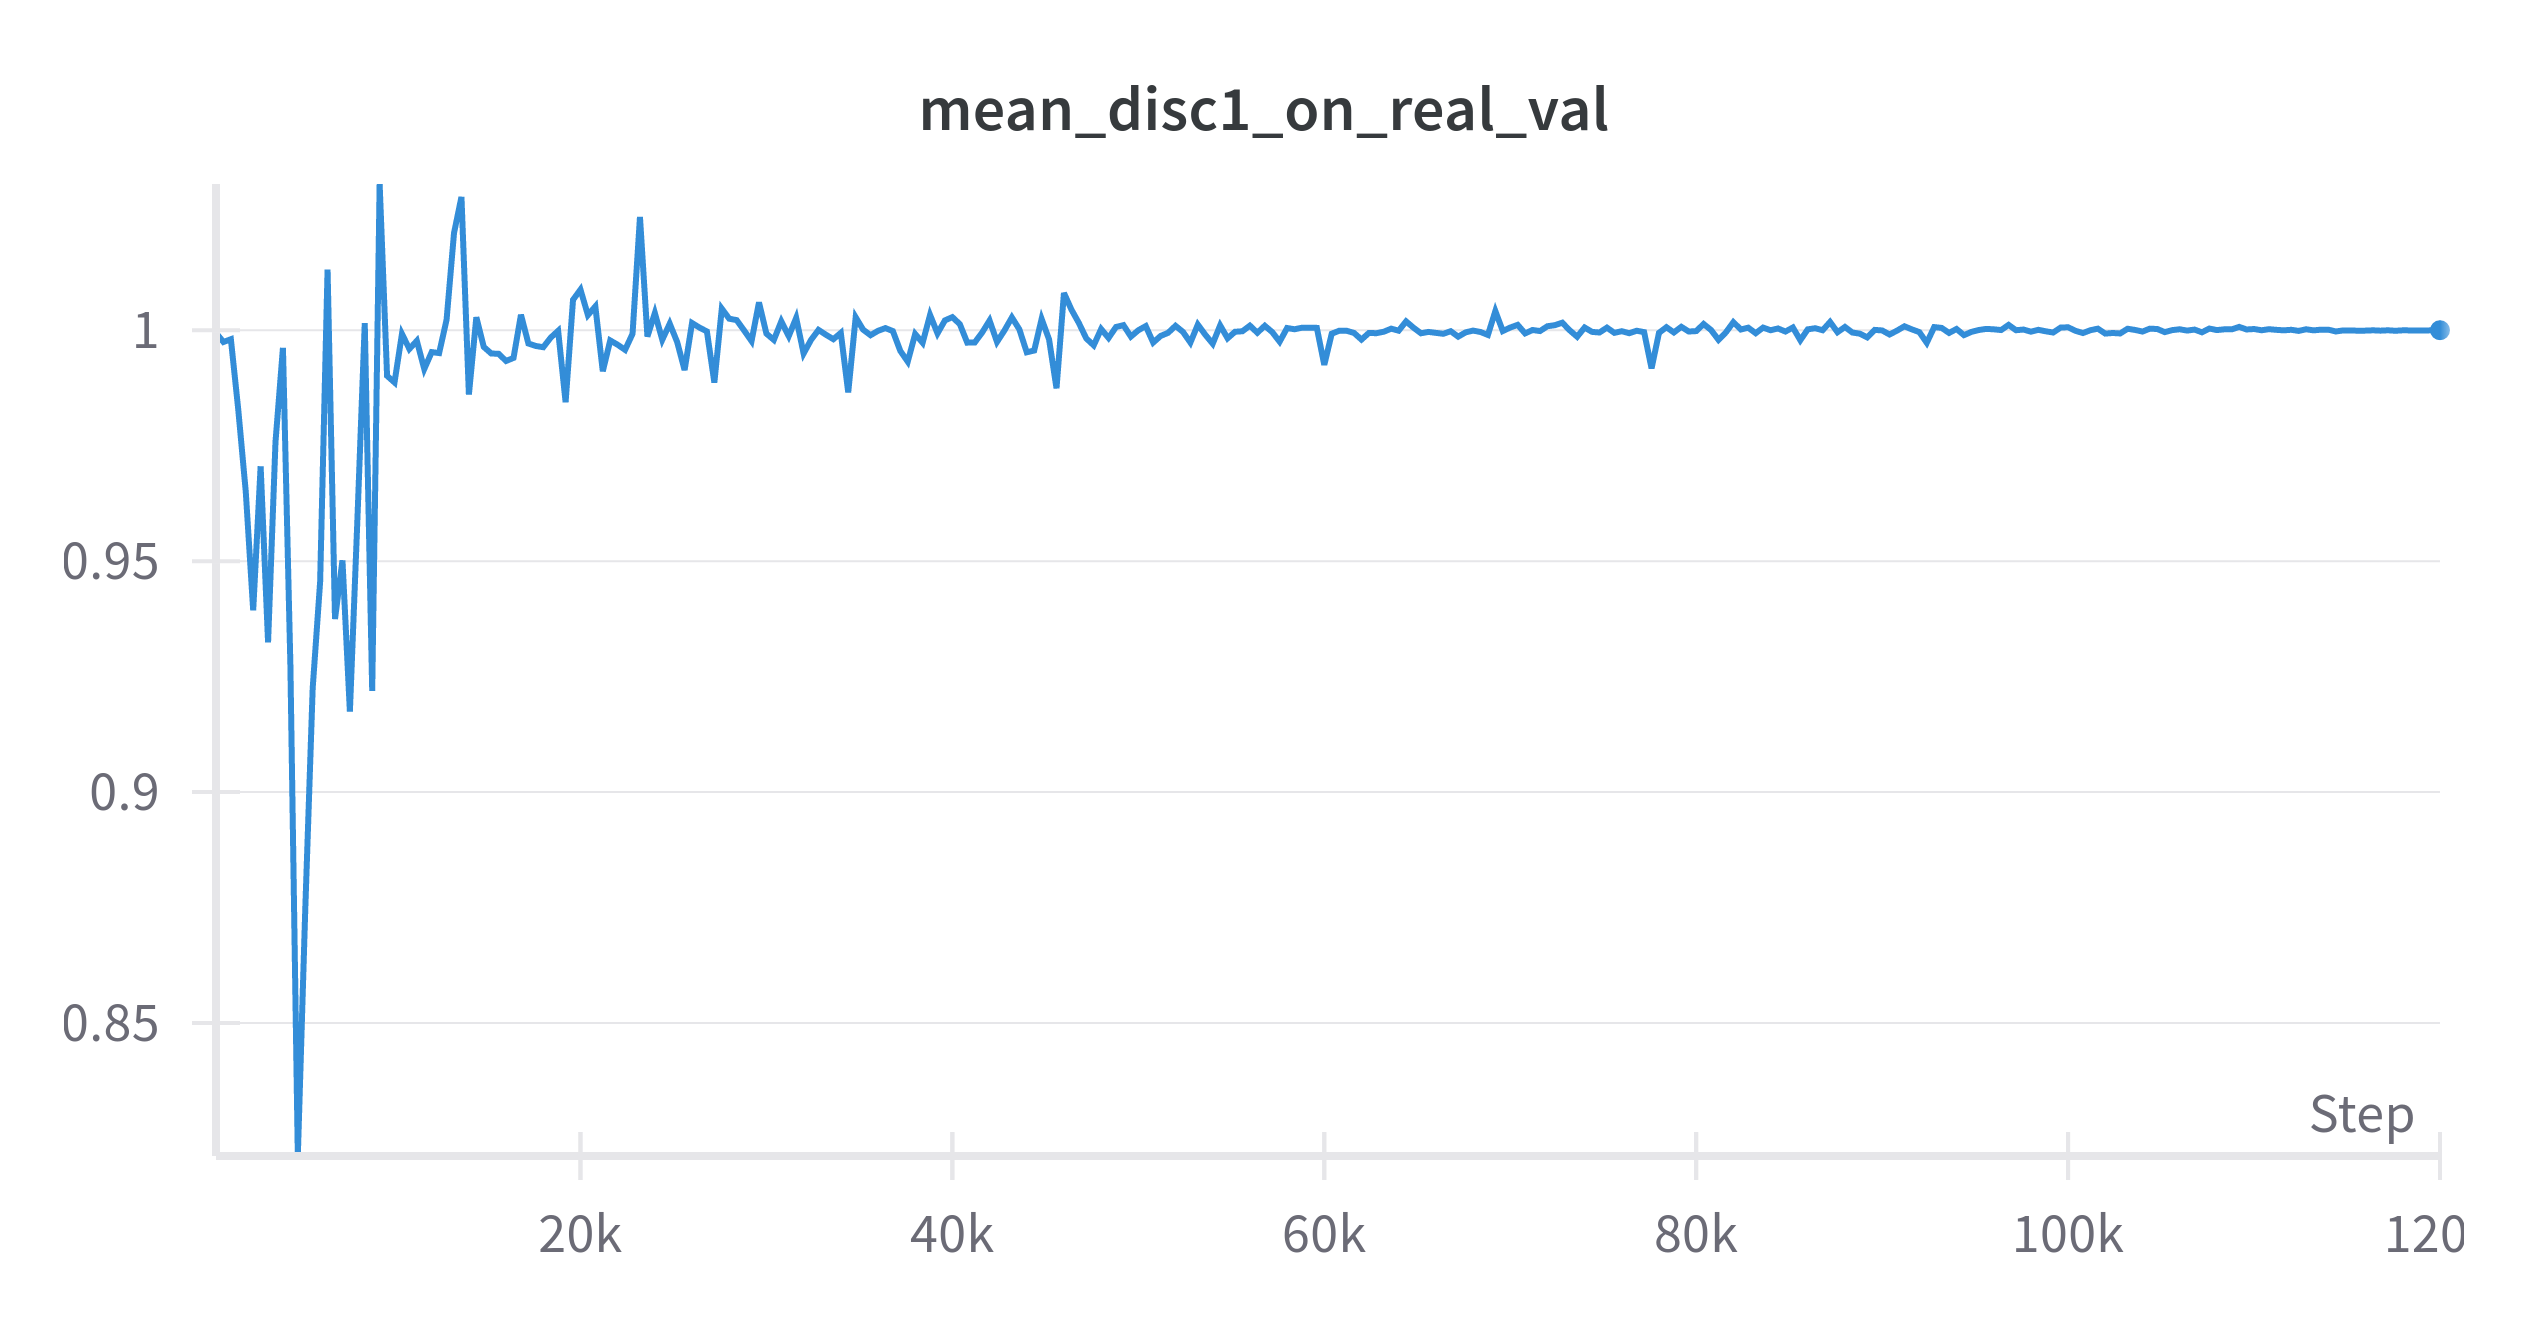
\includegraphics[width=0.4\textwidth]{mean-disc1-on-real-val.png} \\
    (a) & (b) & (c) \\
    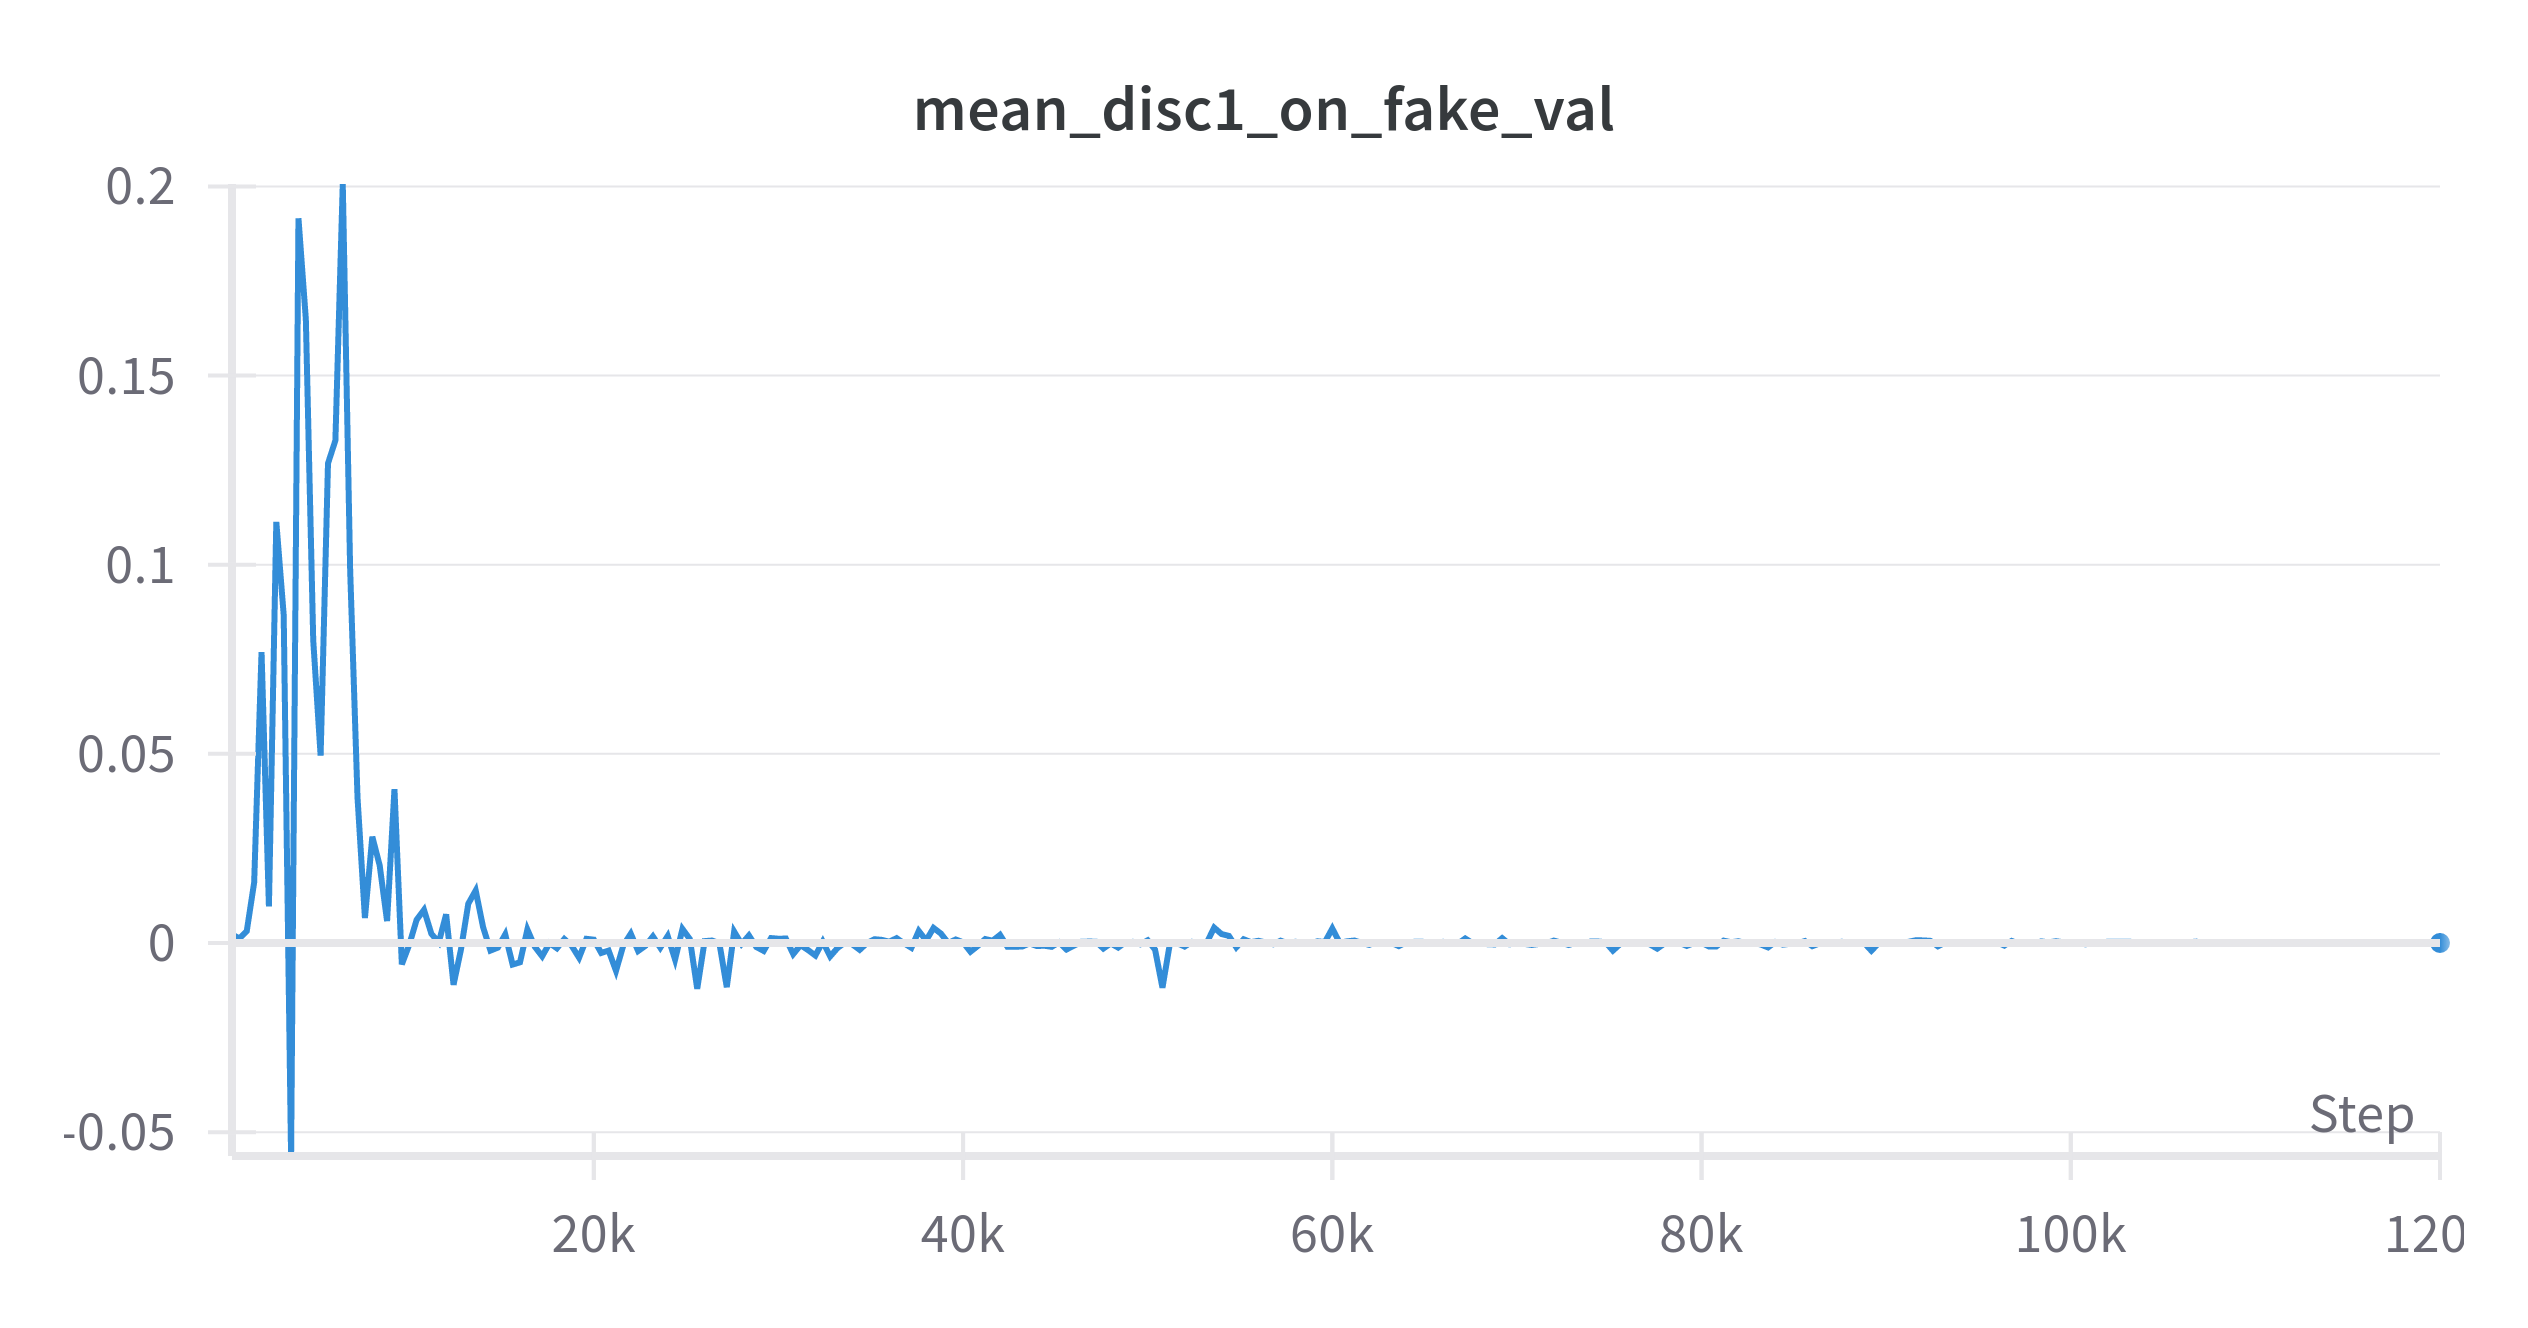
\includegraphics[width=0.4\textwidth]{mean-disc1-on-fake-val.png} &
    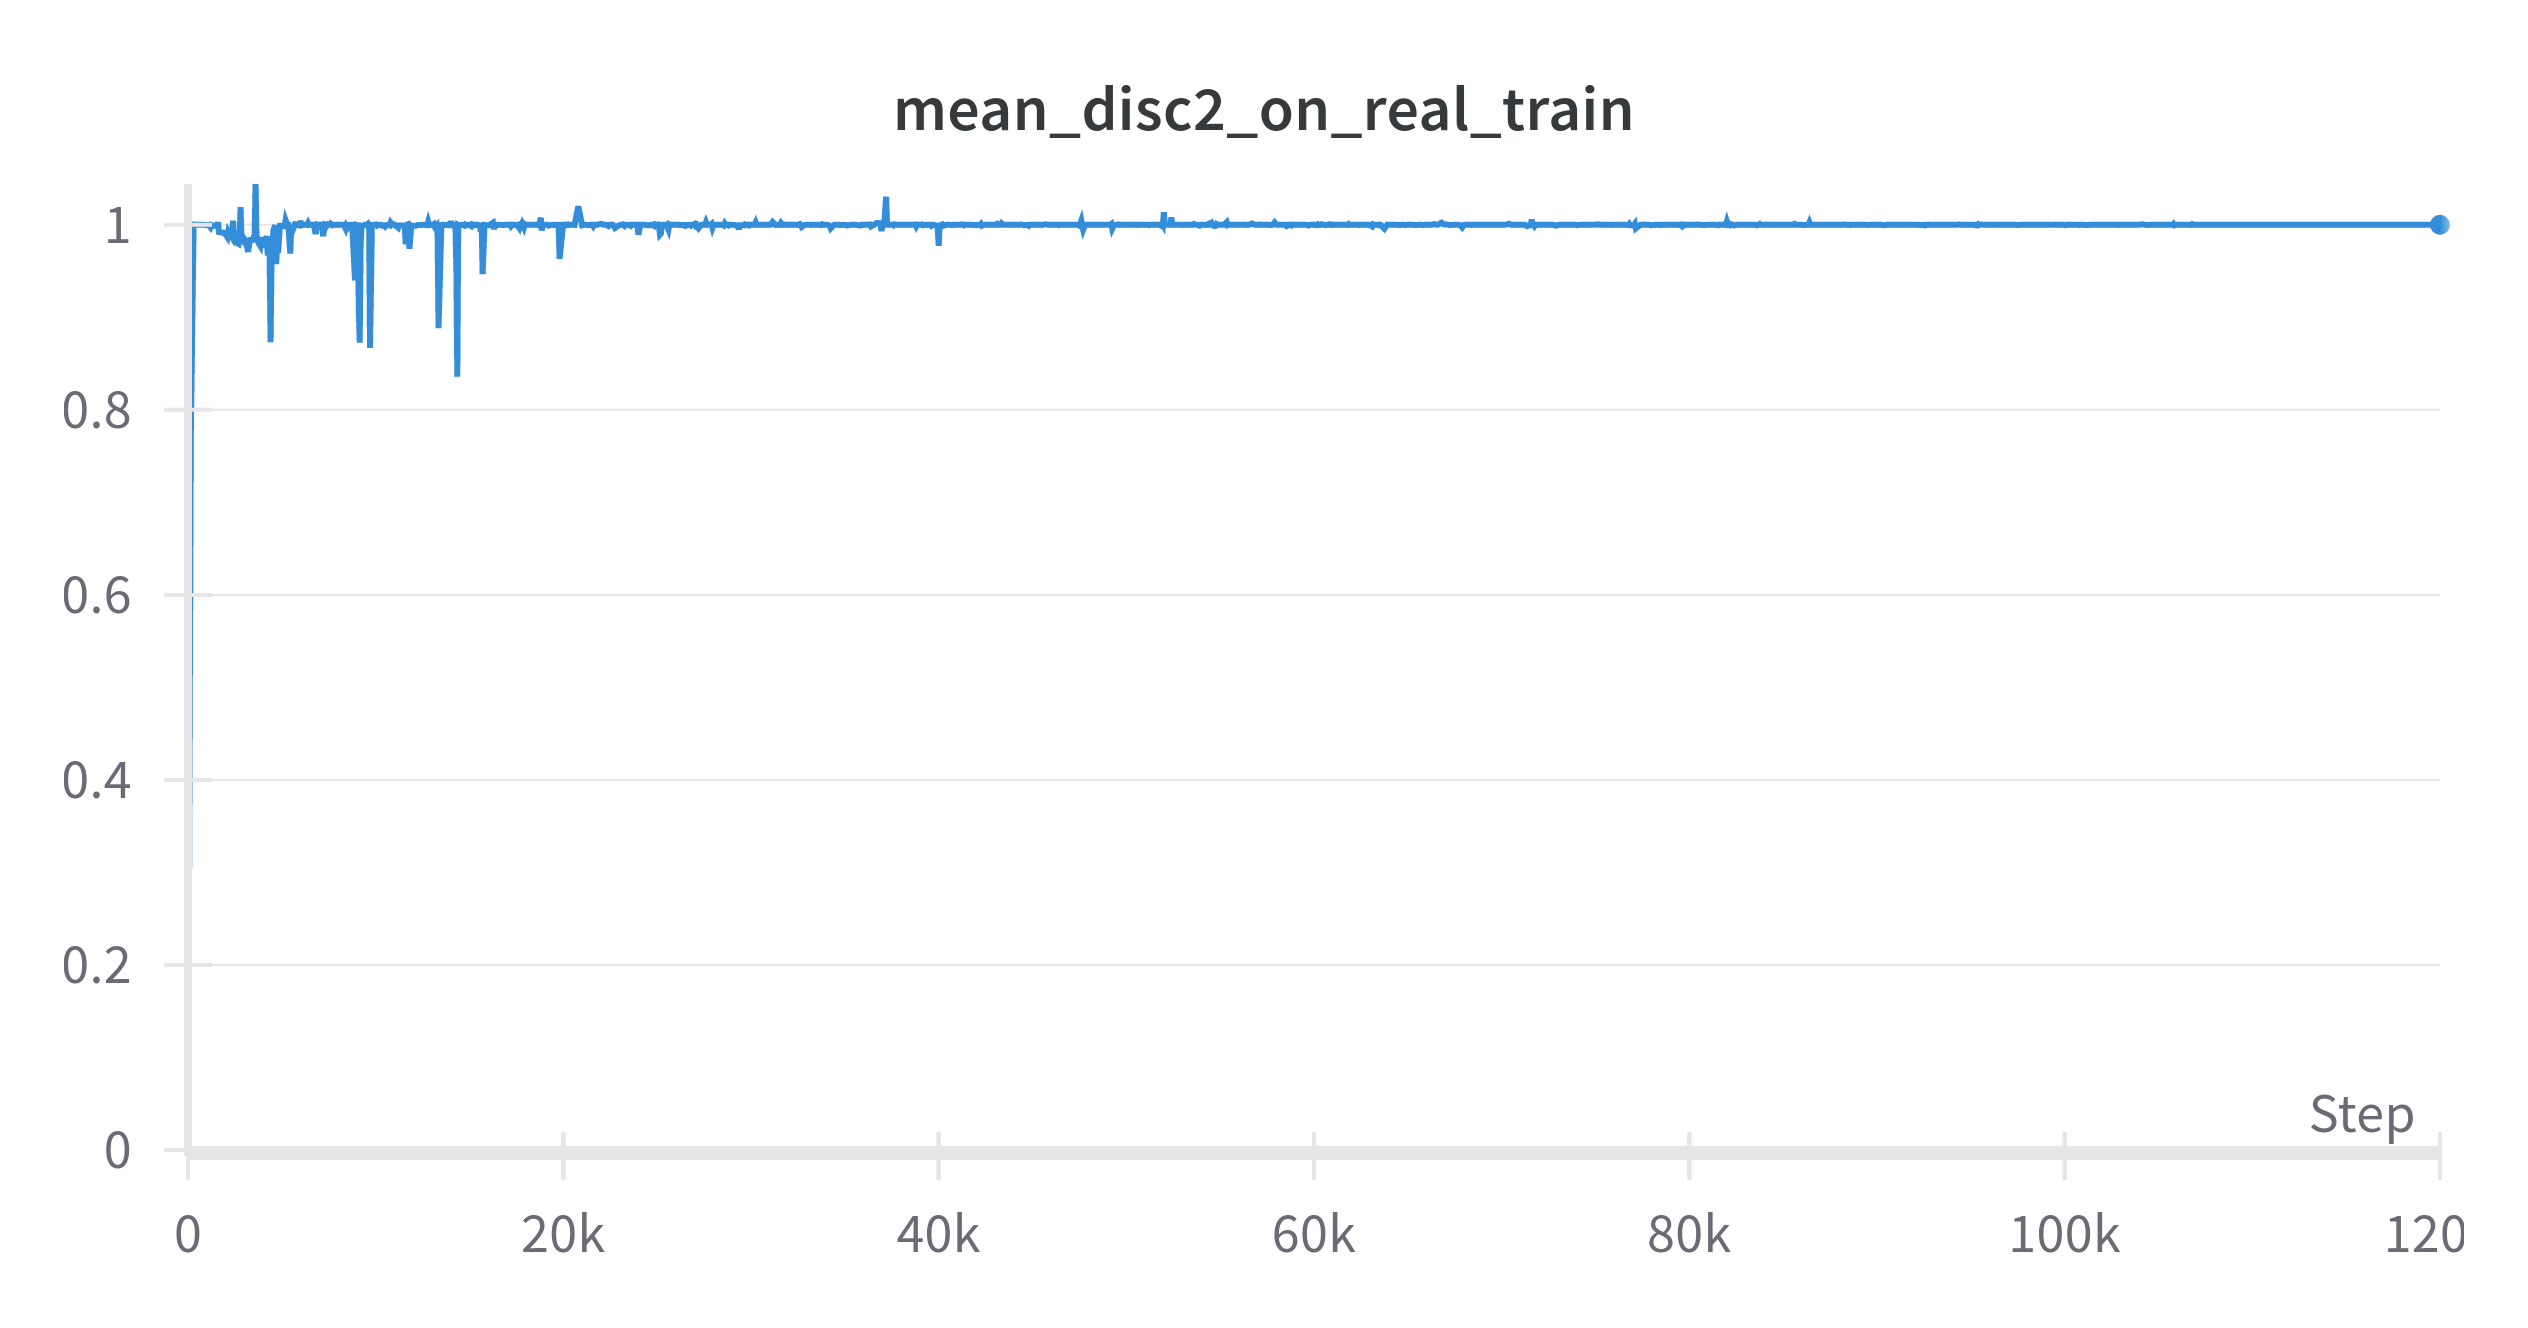
\includegraphics[width=0.4\textwidth]{mean-disc2-on-real-train.png} &
    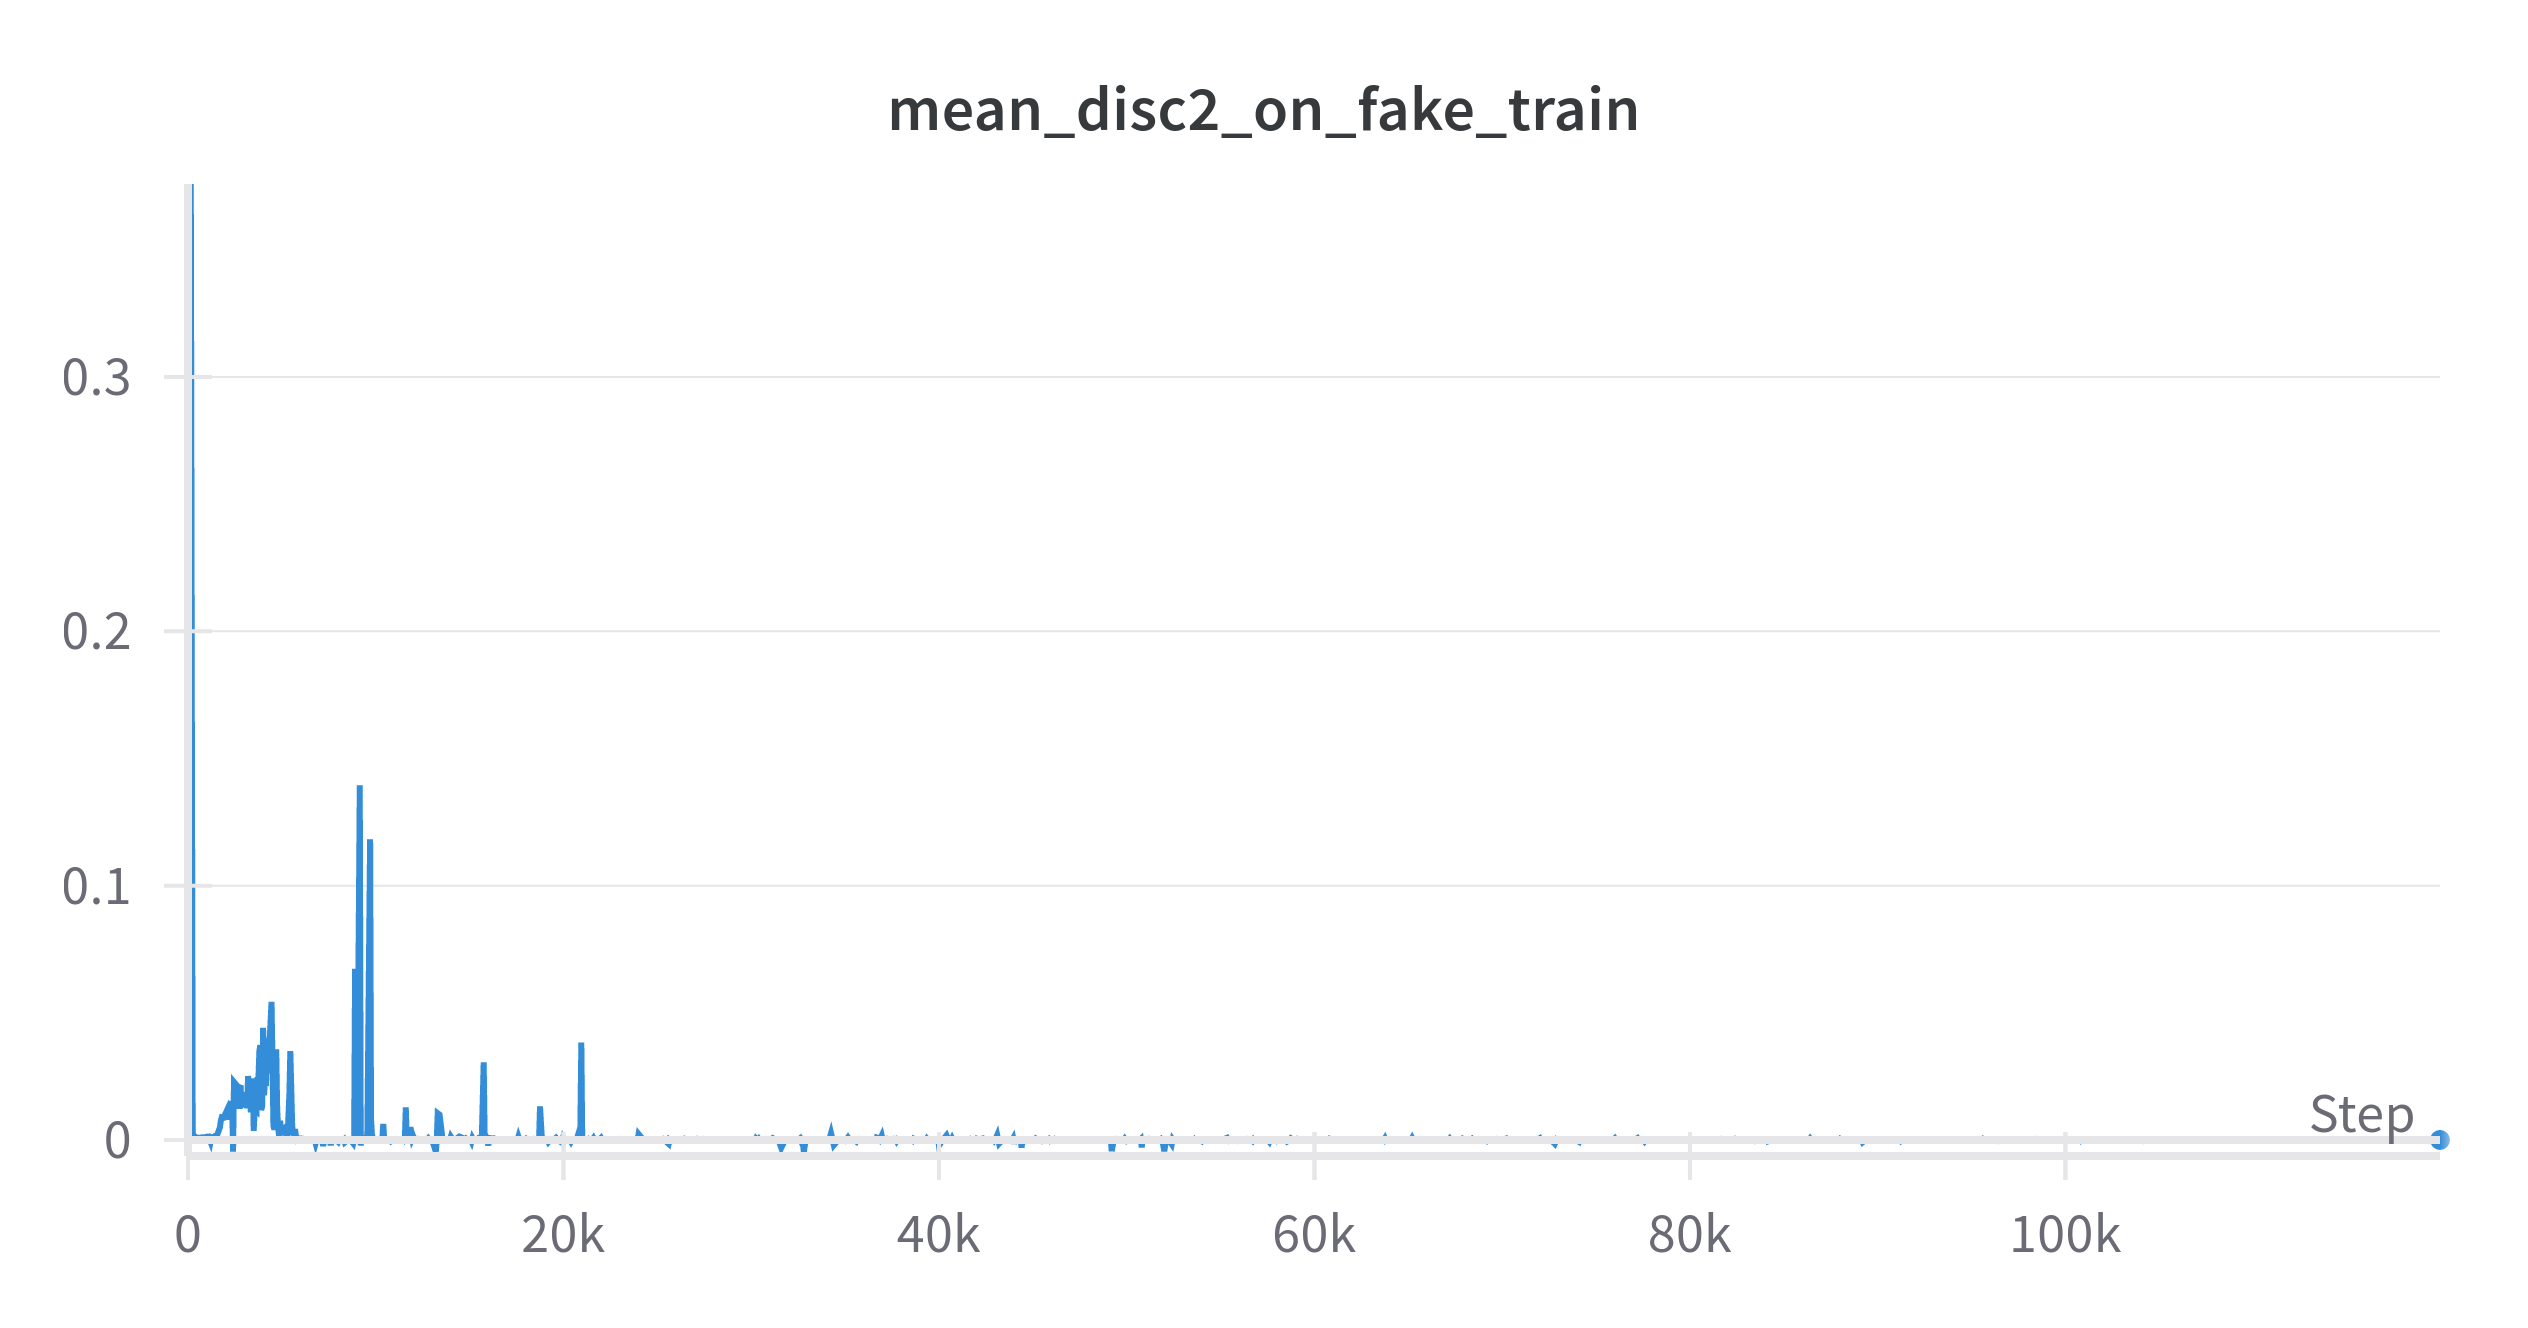
\includegraphics[width=0.4\textwidth]{mean-disc2-on-fake-train.png} \\
    (d) & (e) & (f) \\
    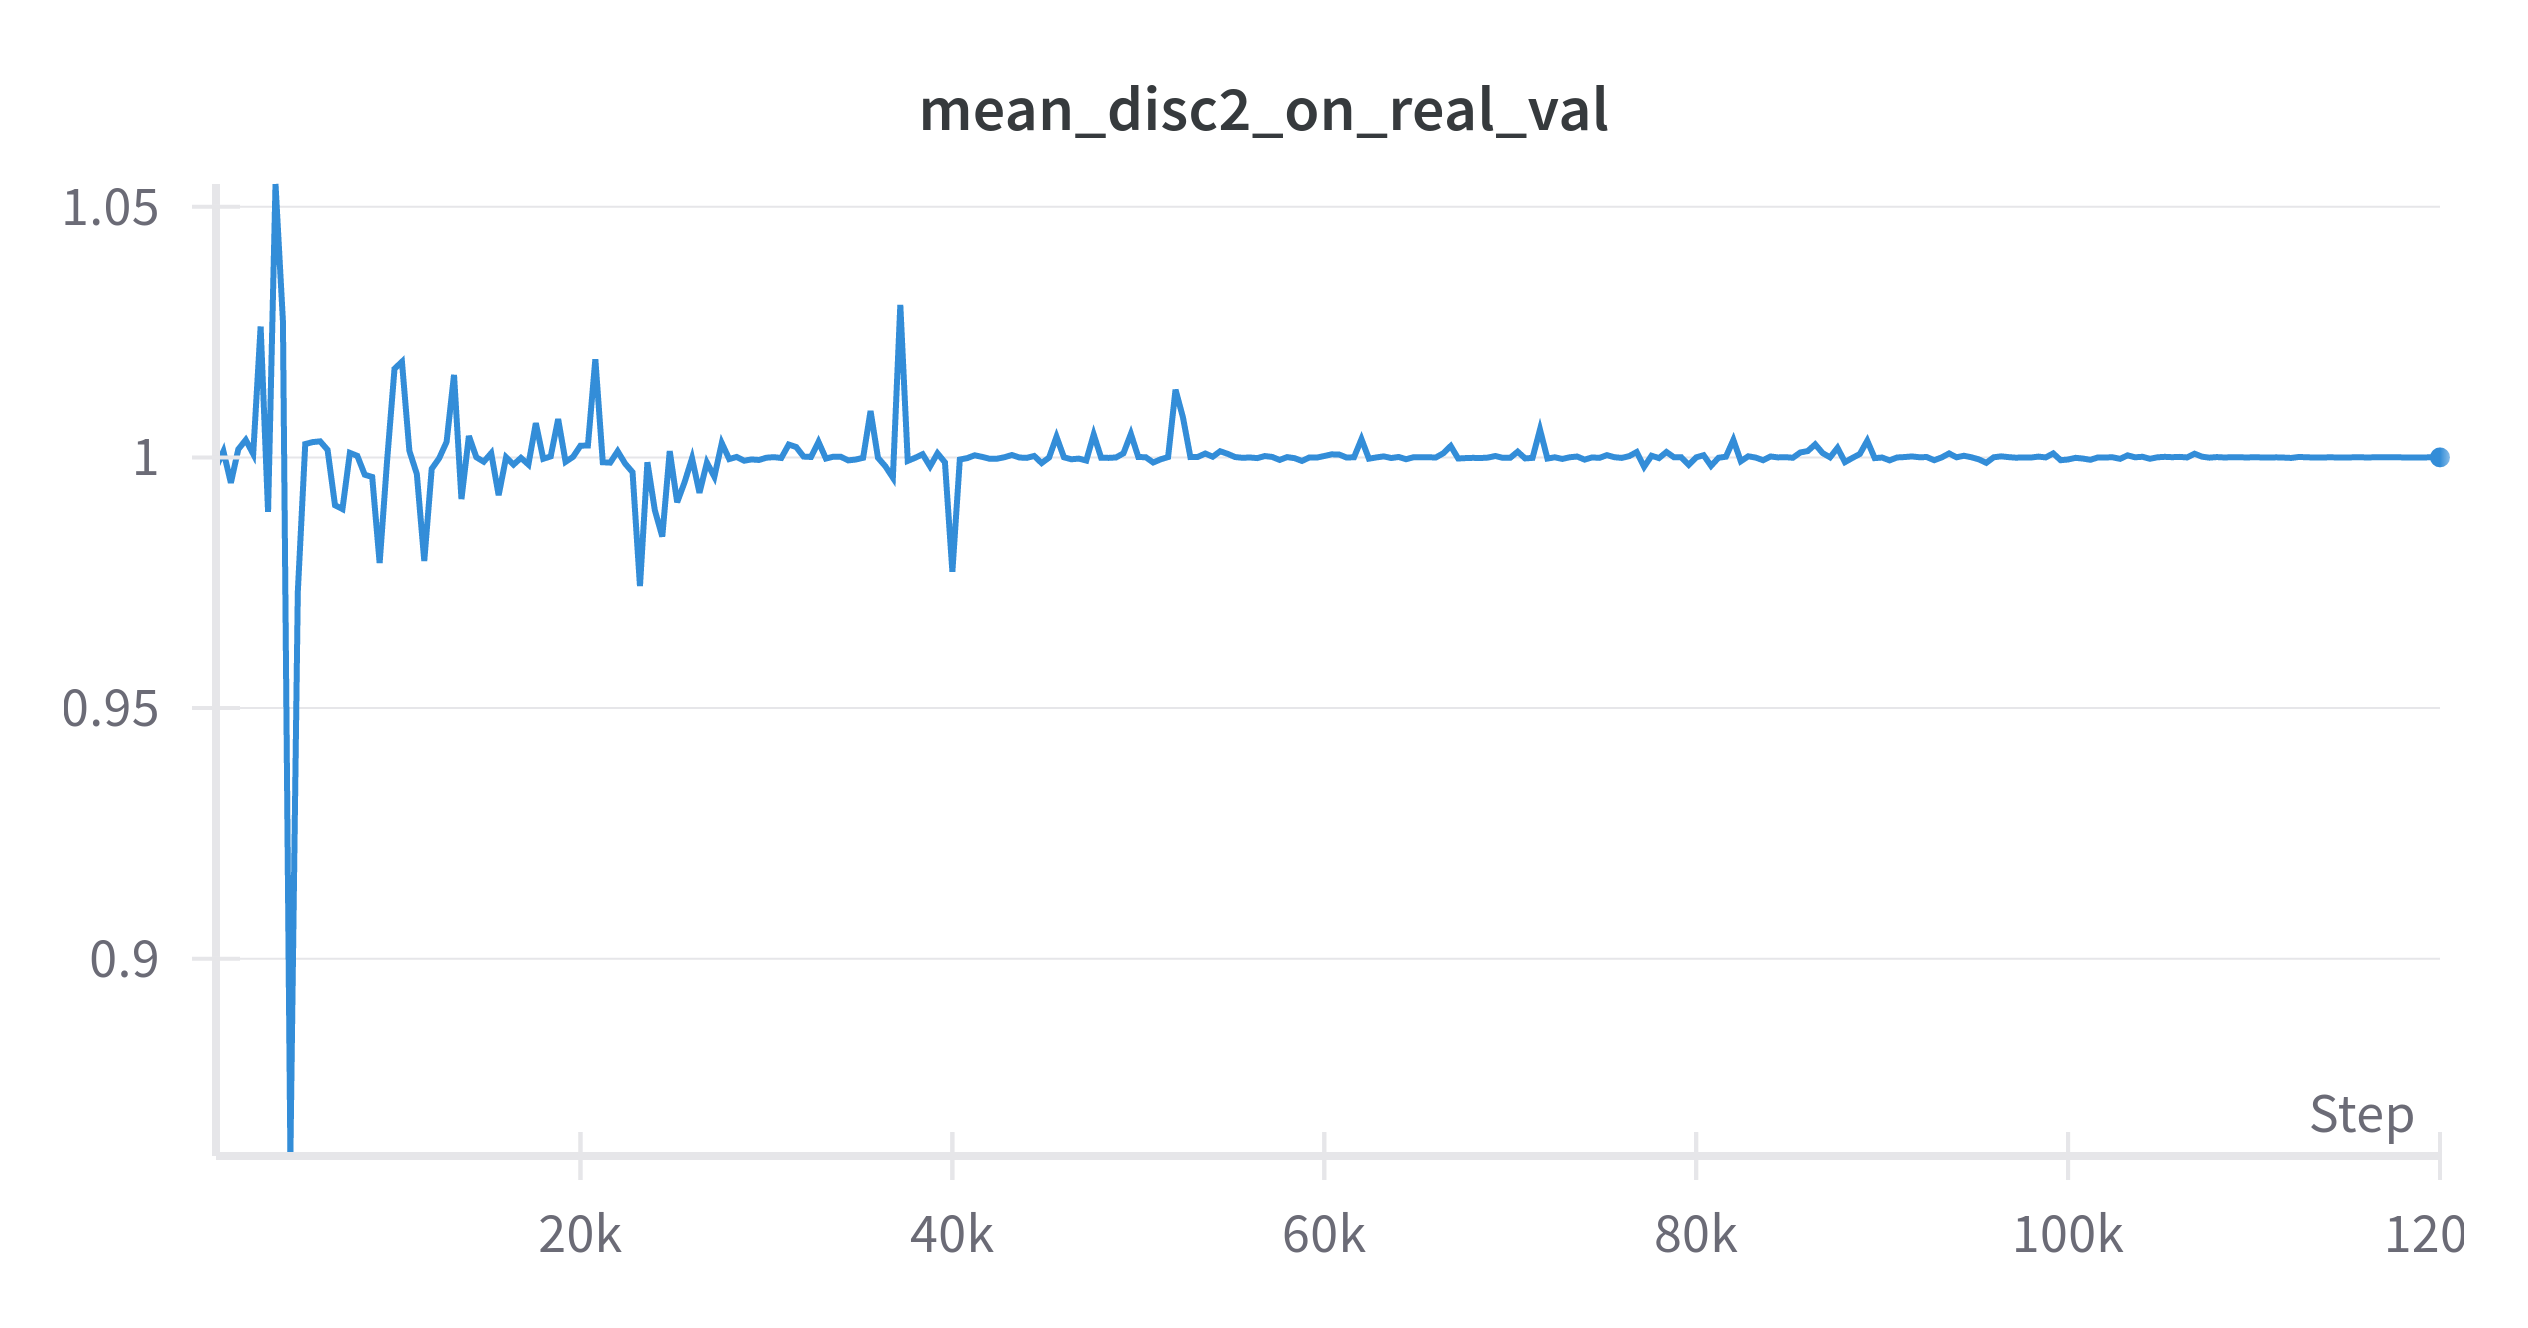
\includegraphics[width=0.4\textwidth]{mean-disc2-on-real-val.png} &
    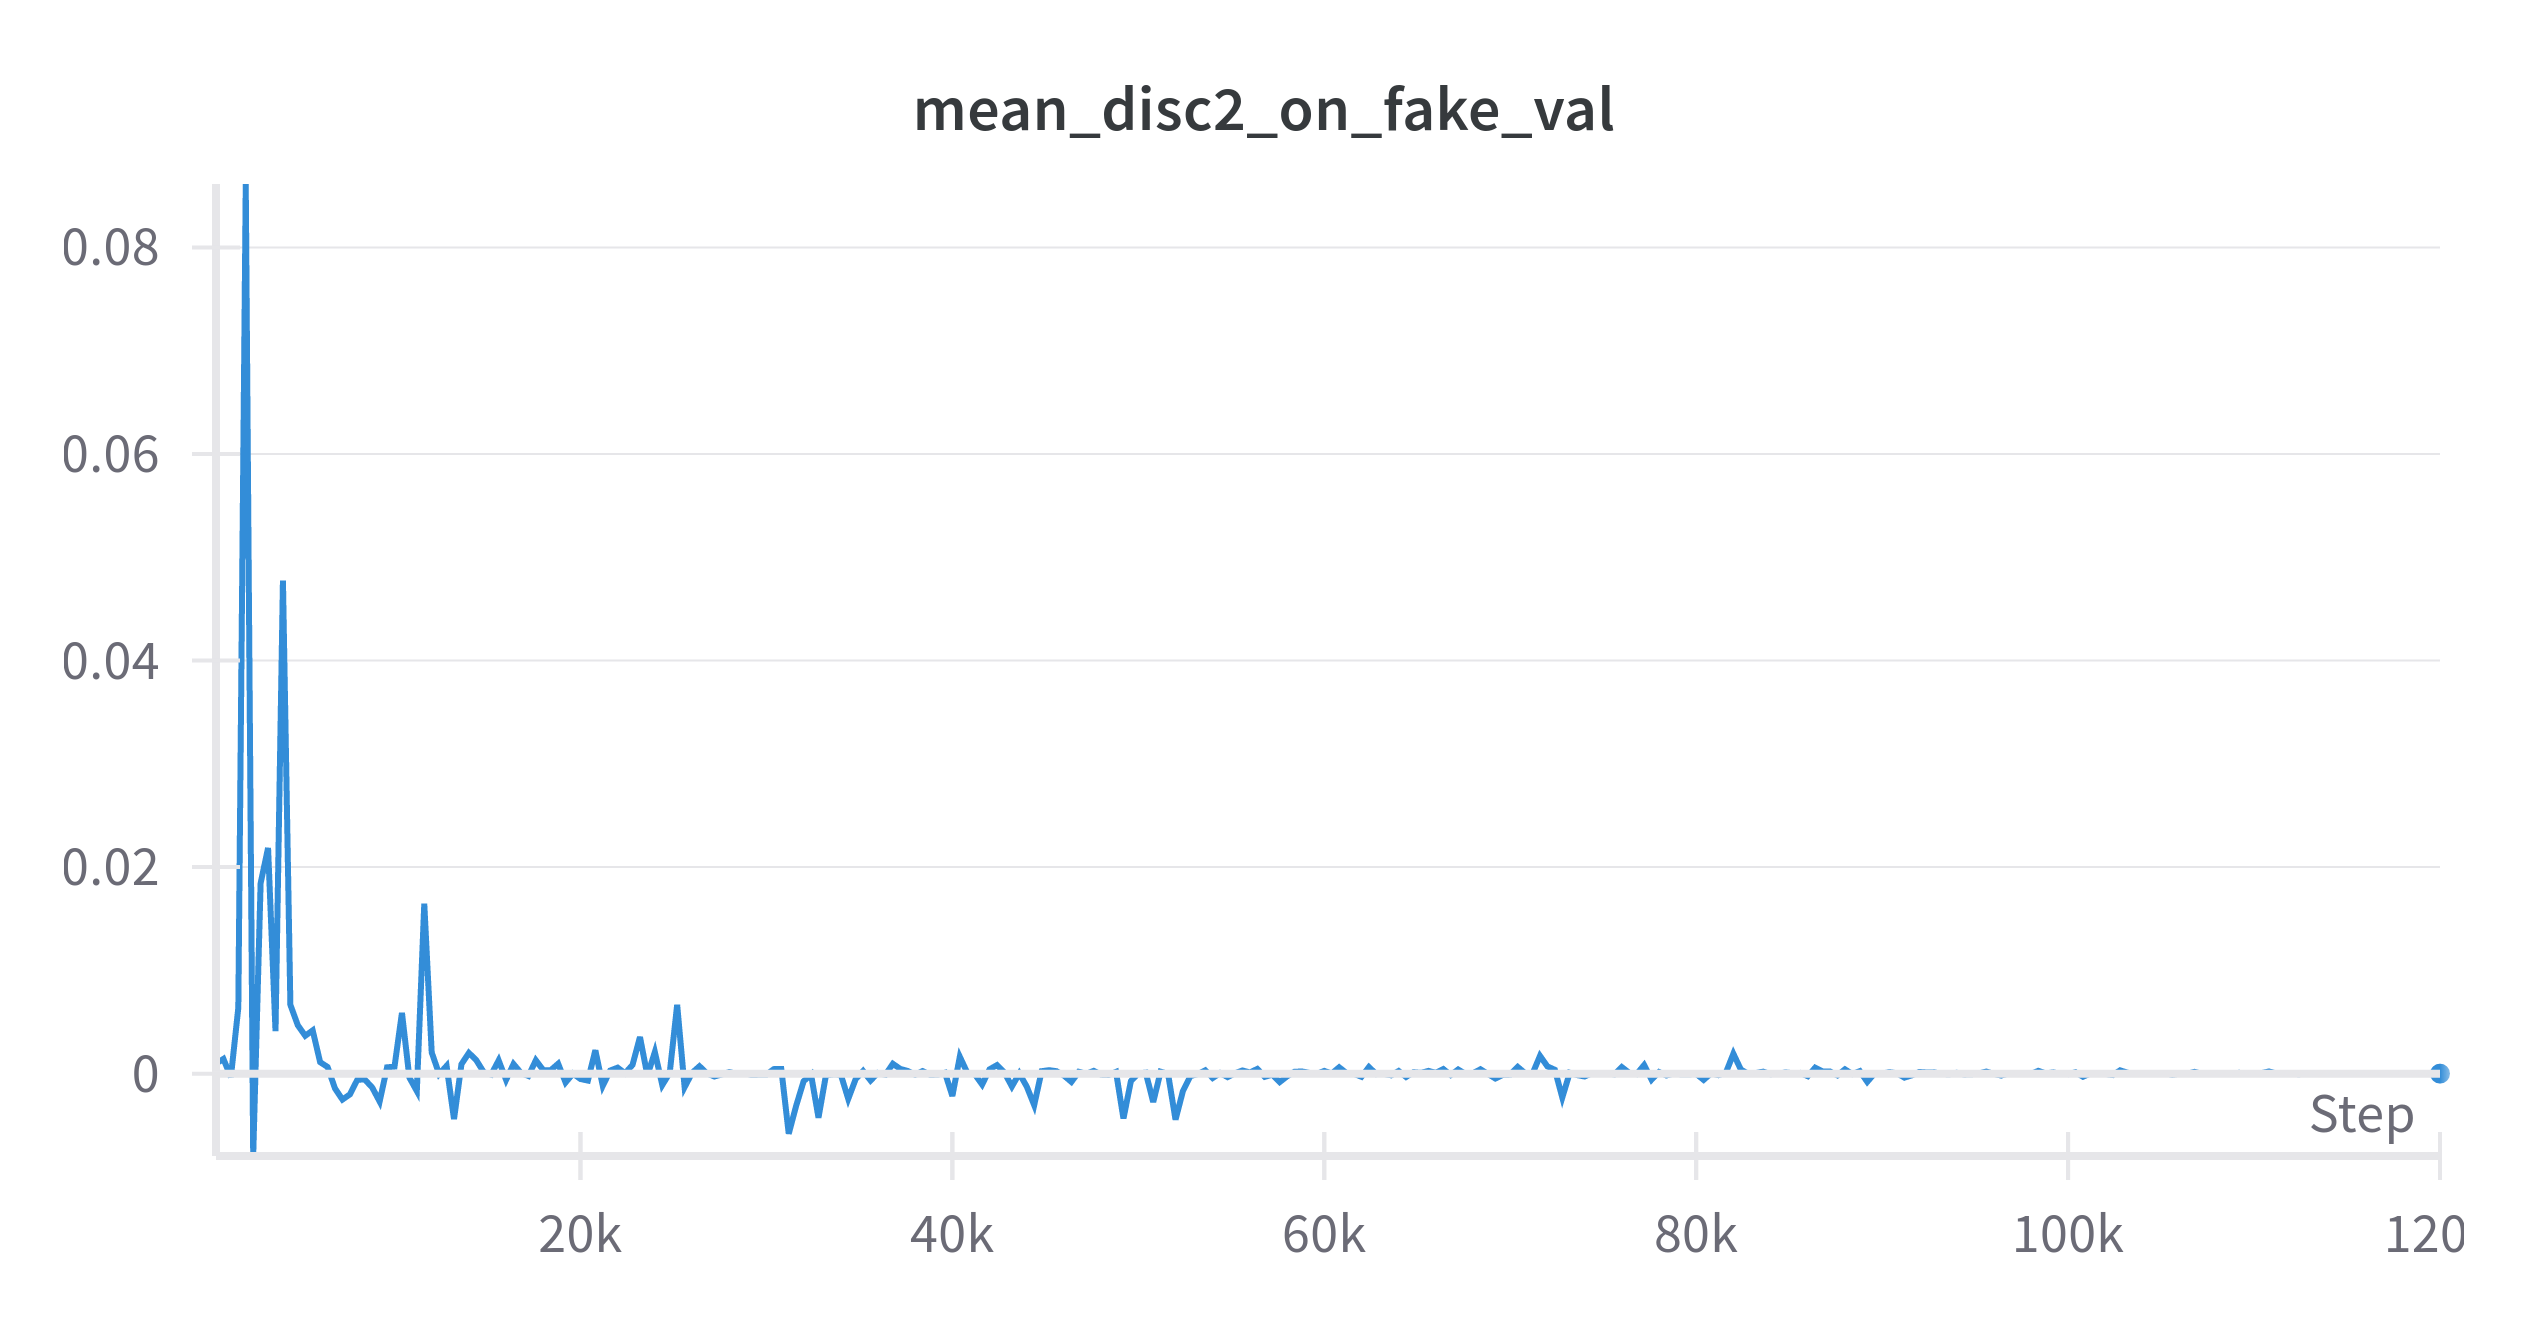
\includegraphics[width=0.4\textwidth]{mean-disc2-on-fake-val.png} &
  \end{tabular}
  \caption{Discriminator Mean Outputs on Real and Fake Data during Training and Validation}
  \label{tab:mean-disc-output}
\end{table}

\begin{table}[H]
  \centering
  \begin{tabular}{cc}
    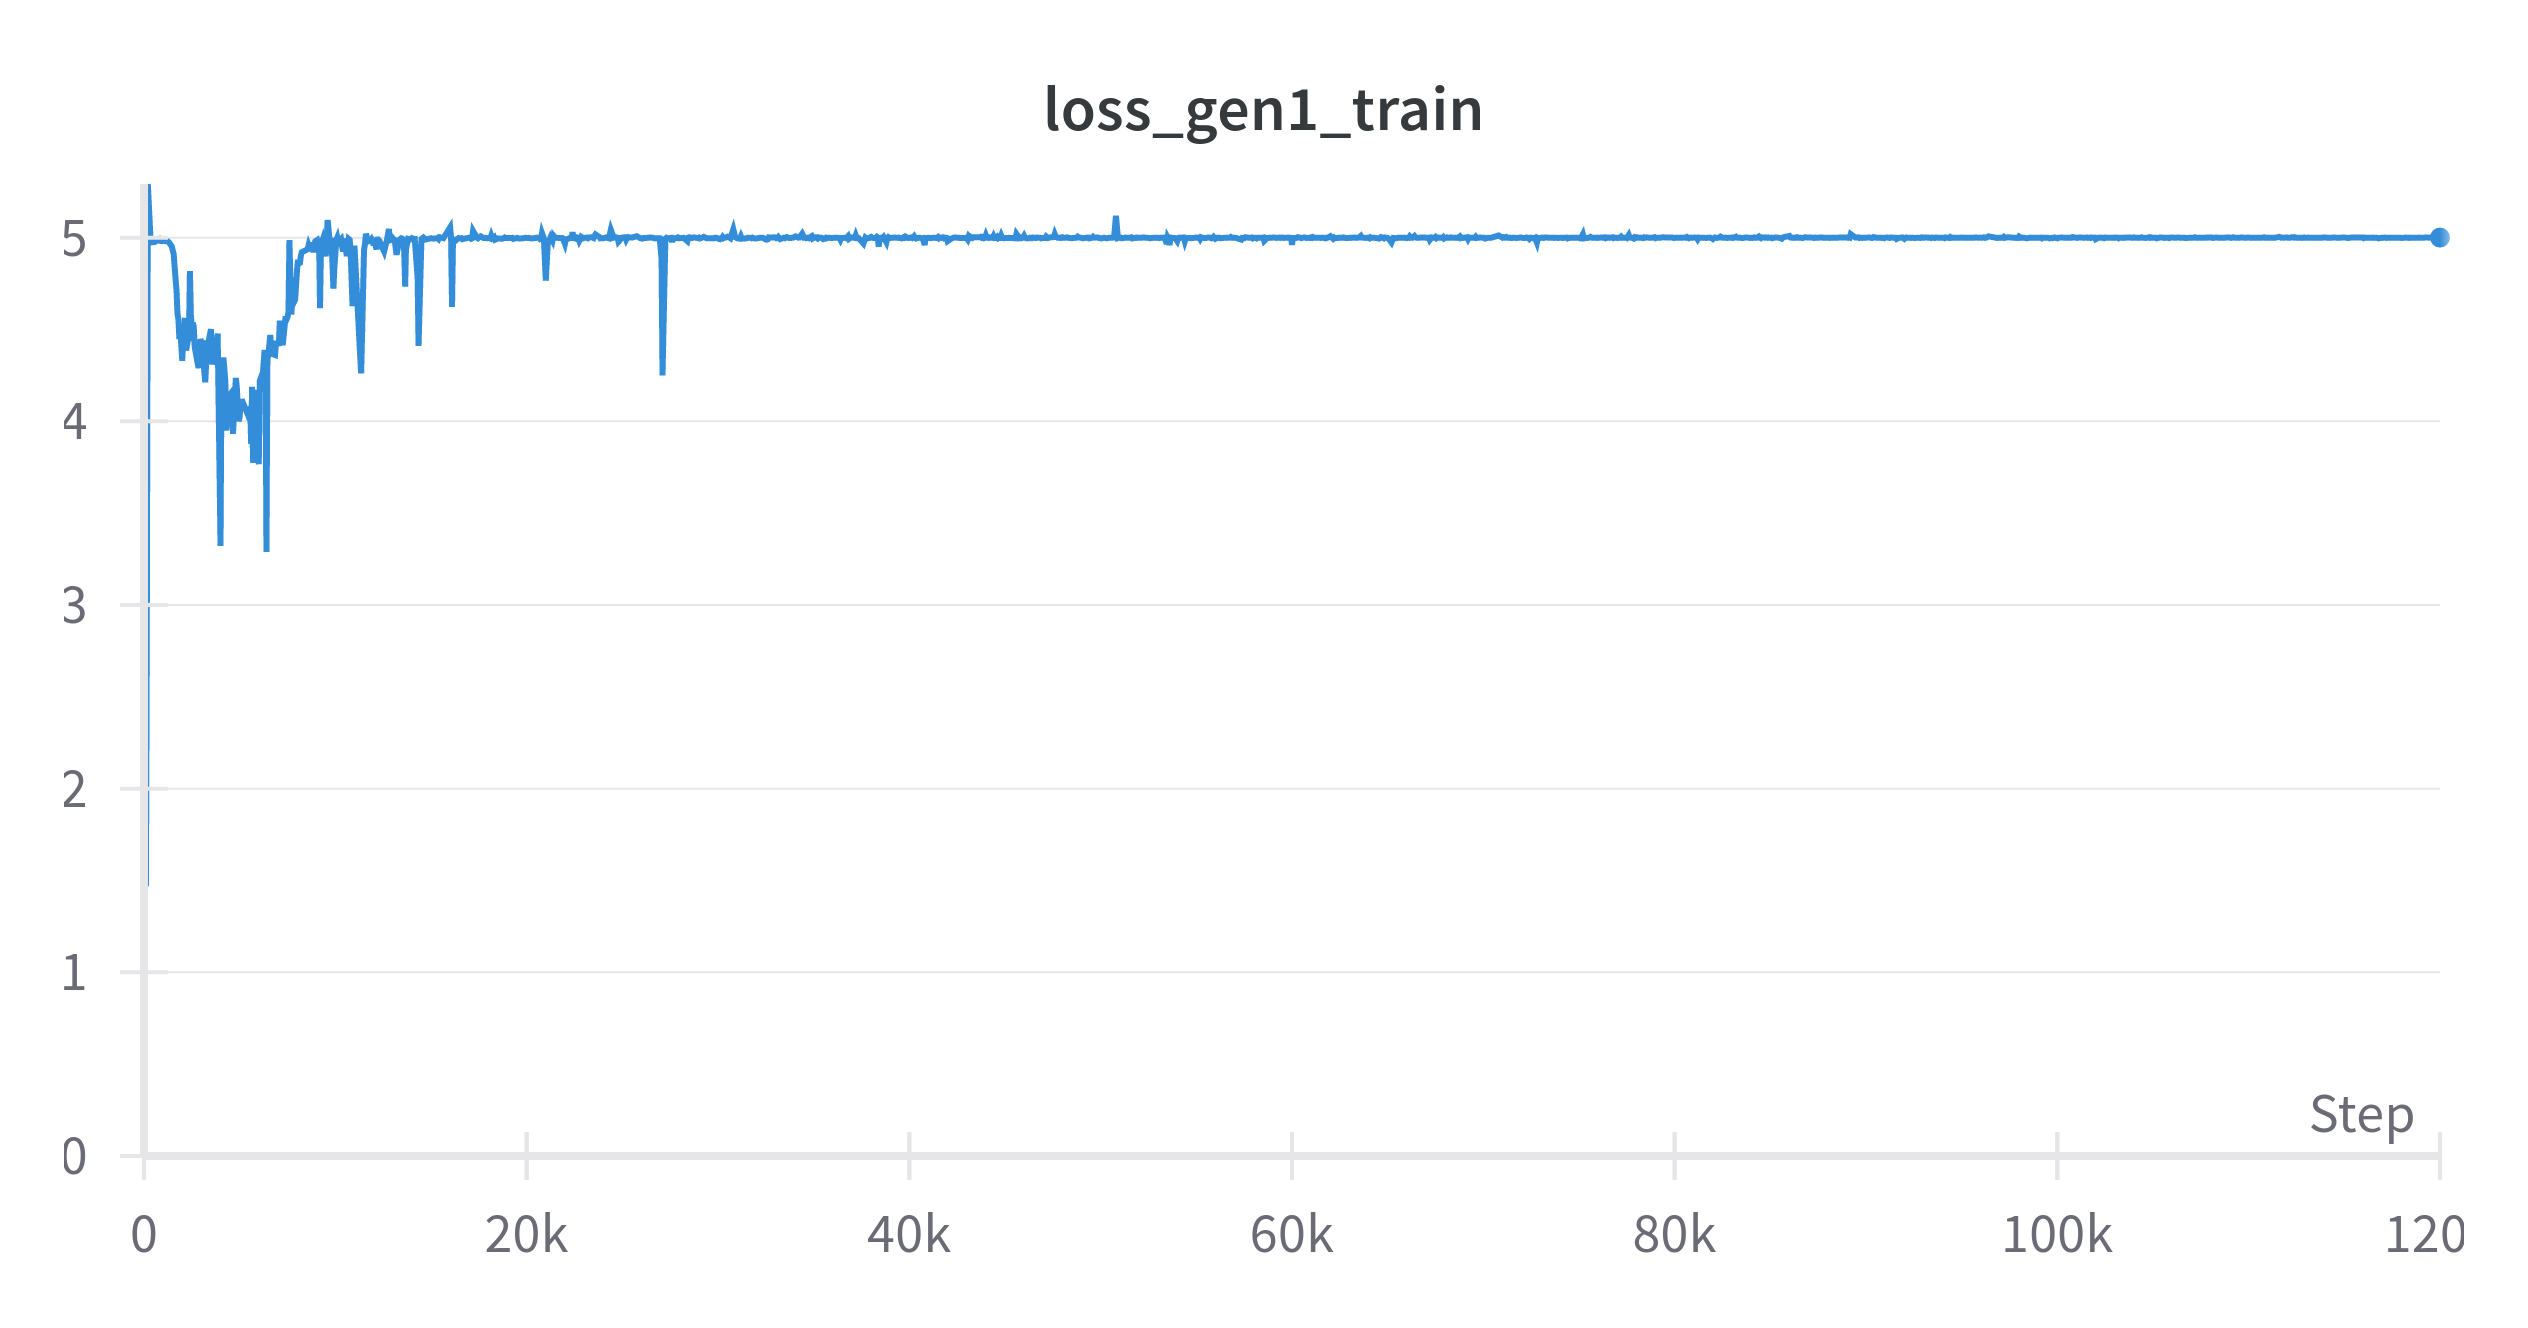
\includegraphics[width=0.4\textwidth]{loss-gen1-train.png} &
    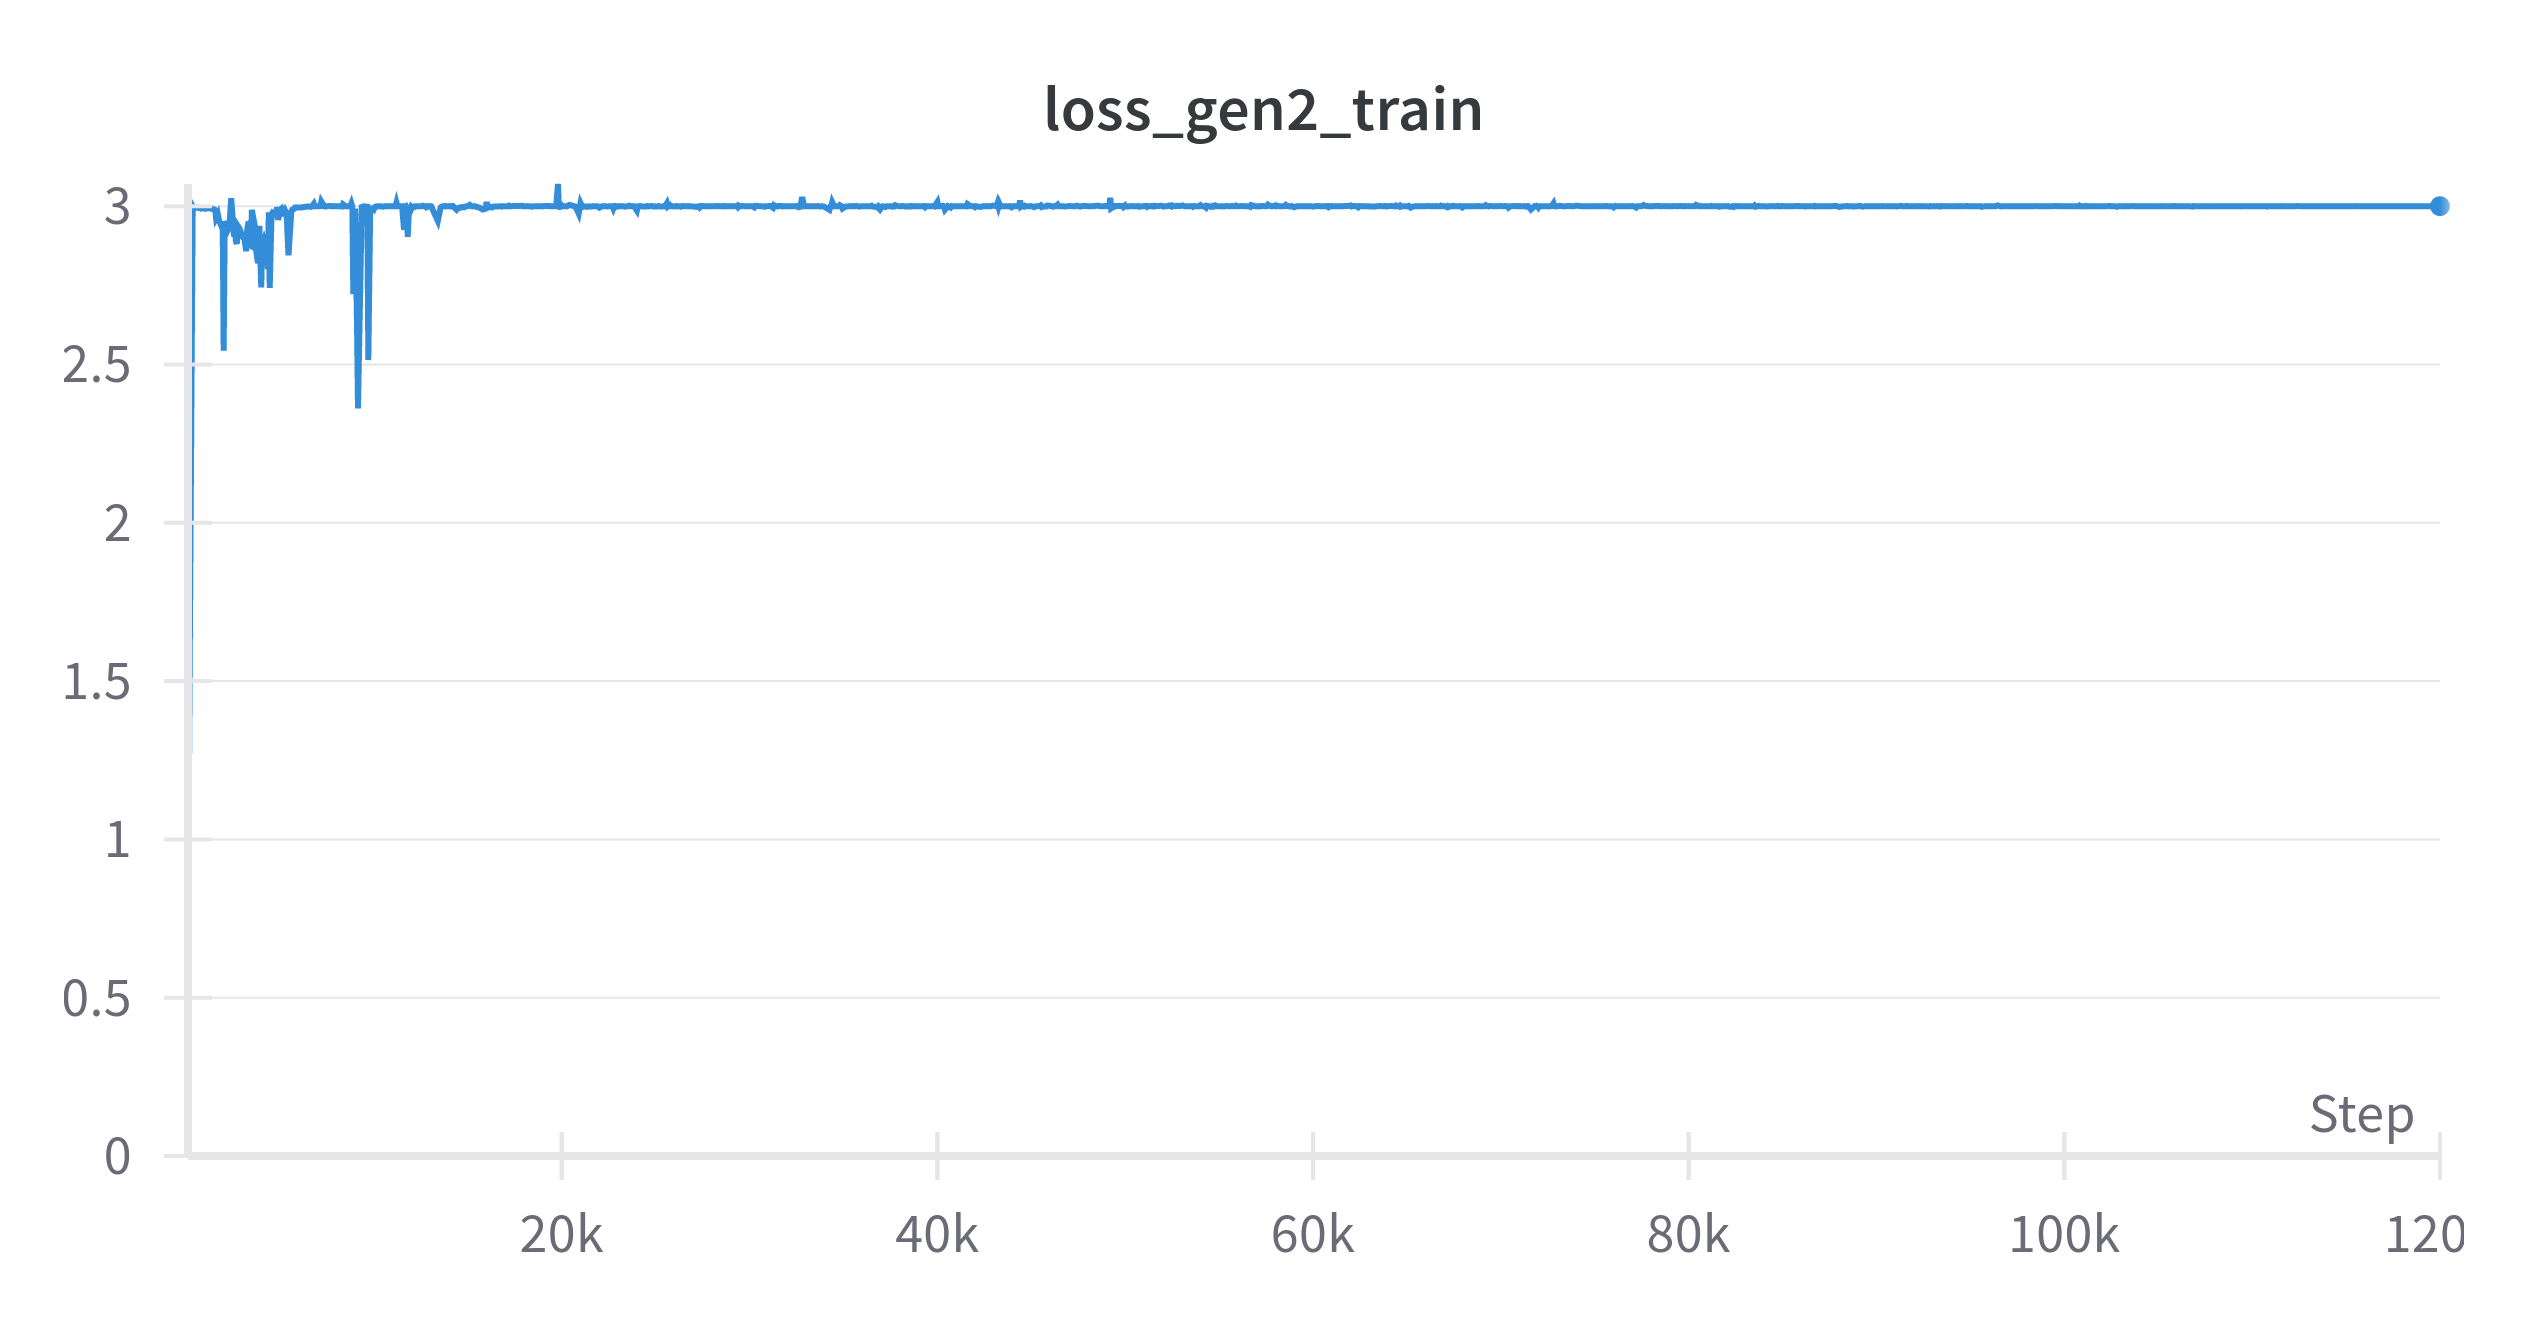
\includegraphics[width=0.4\textwidth]{loss-gen2-train.png} \\
    (a) & (b) \\
    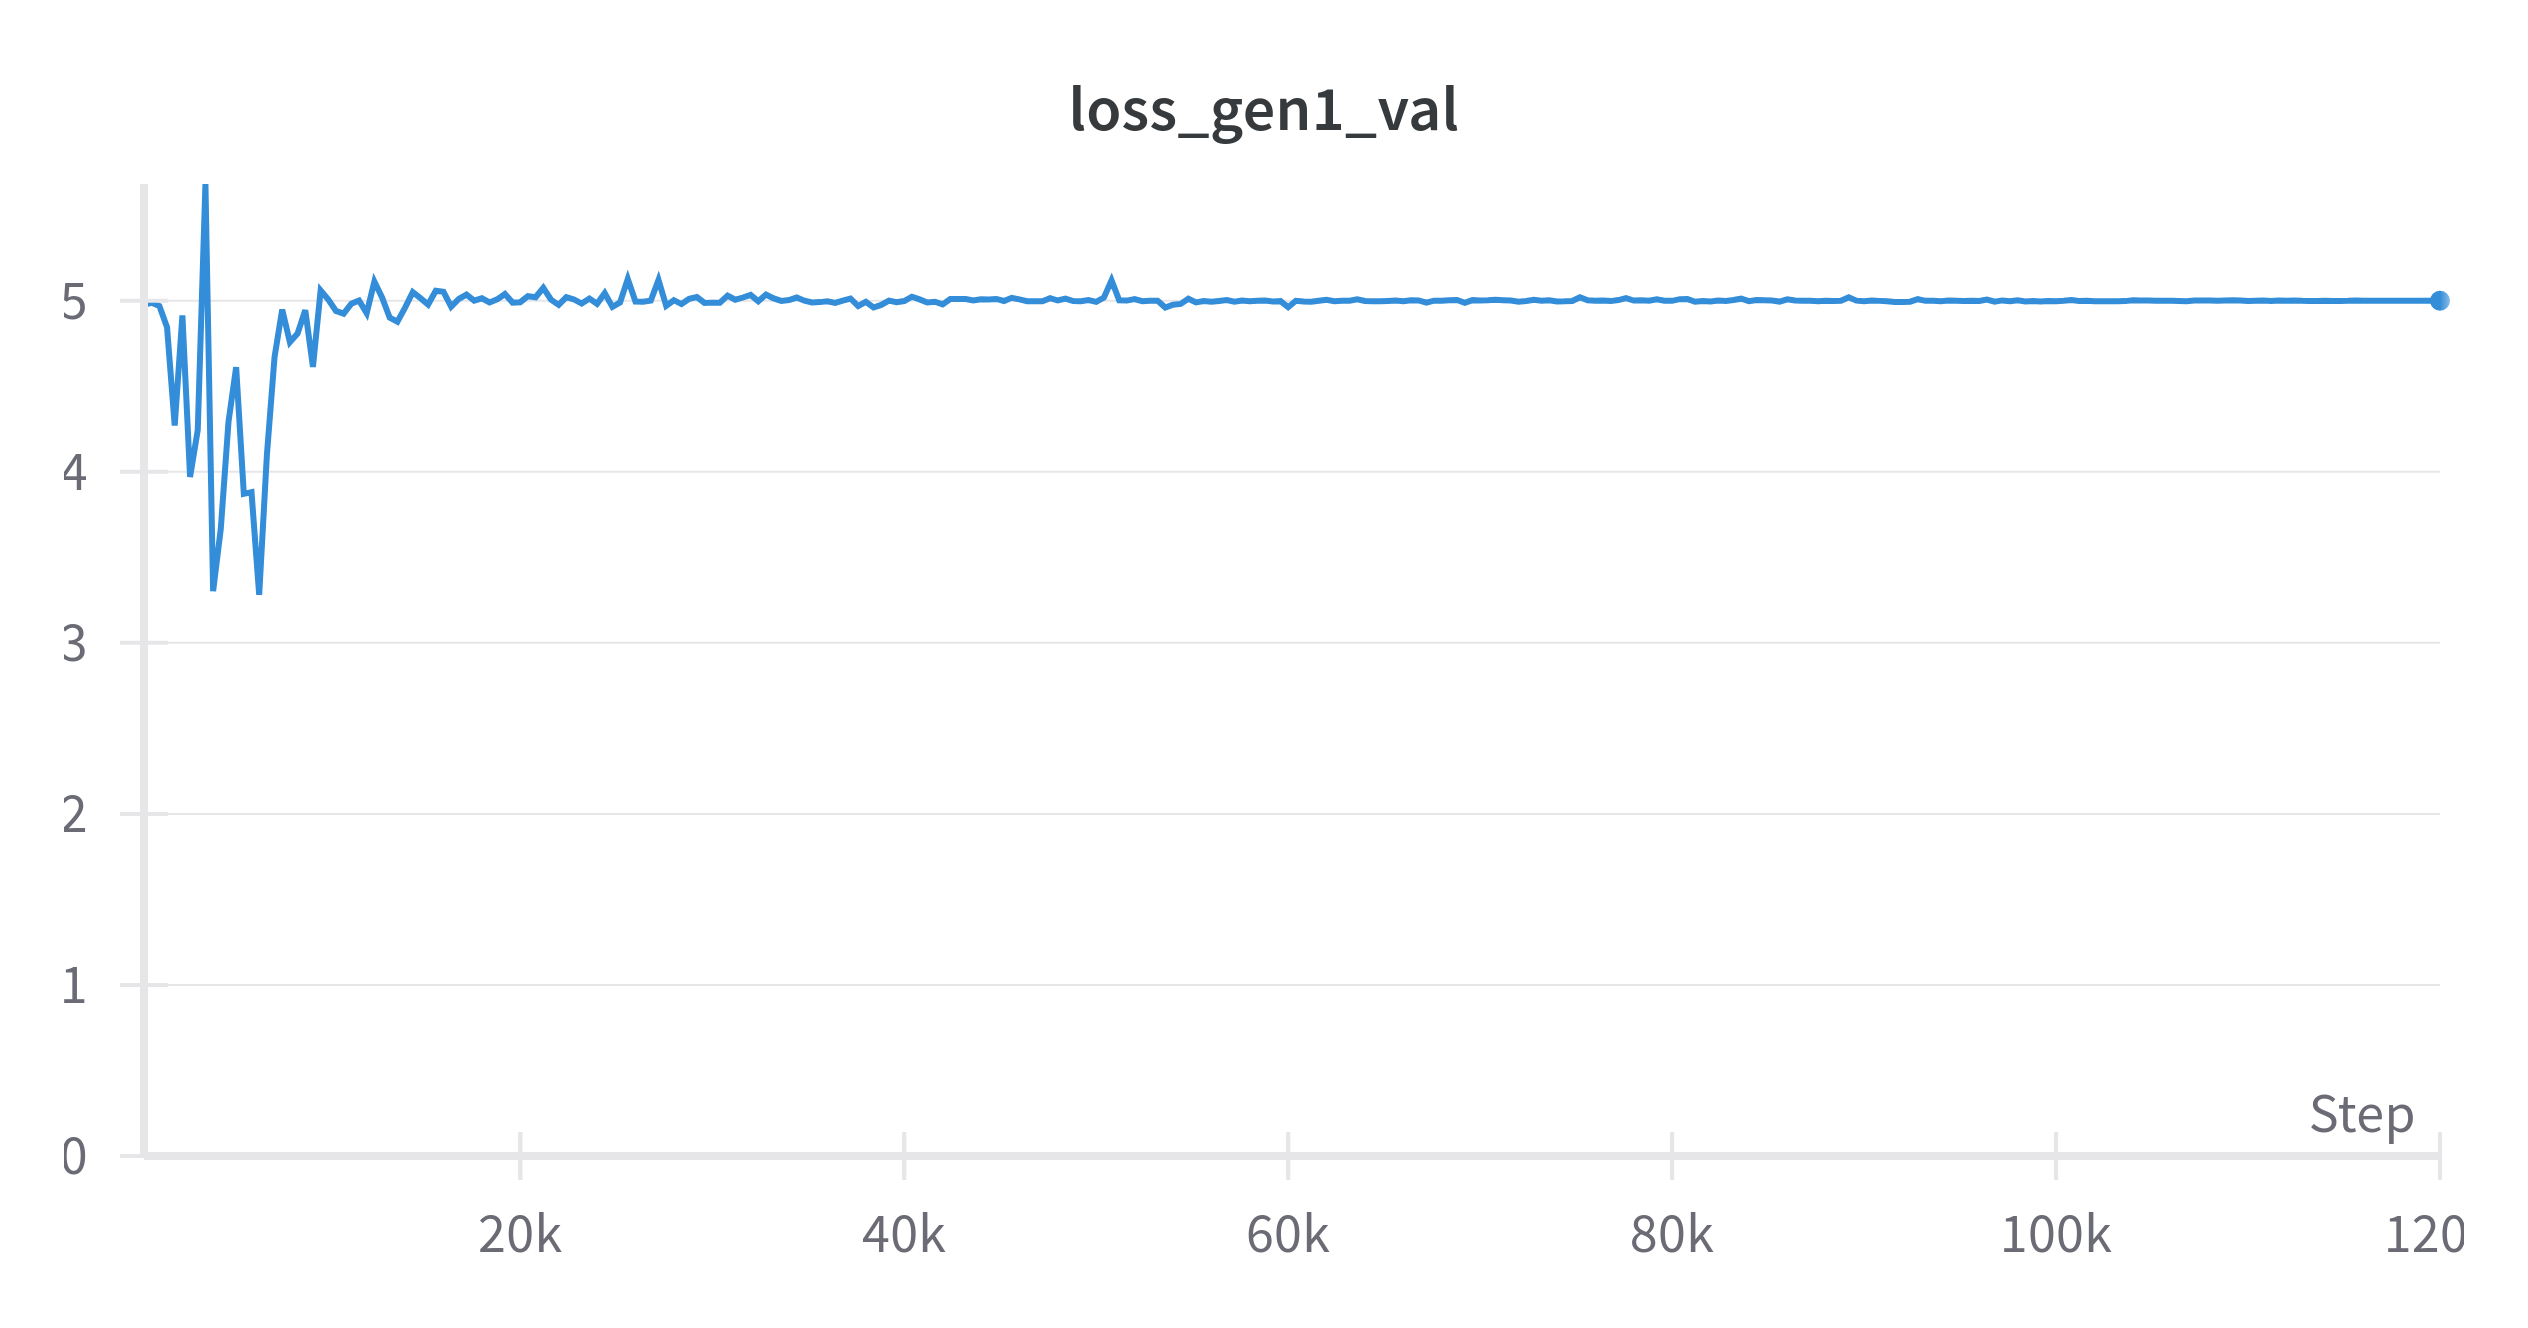
\includegraphics[width=0.4\textwidth]{loss-gen1-val.png} &
    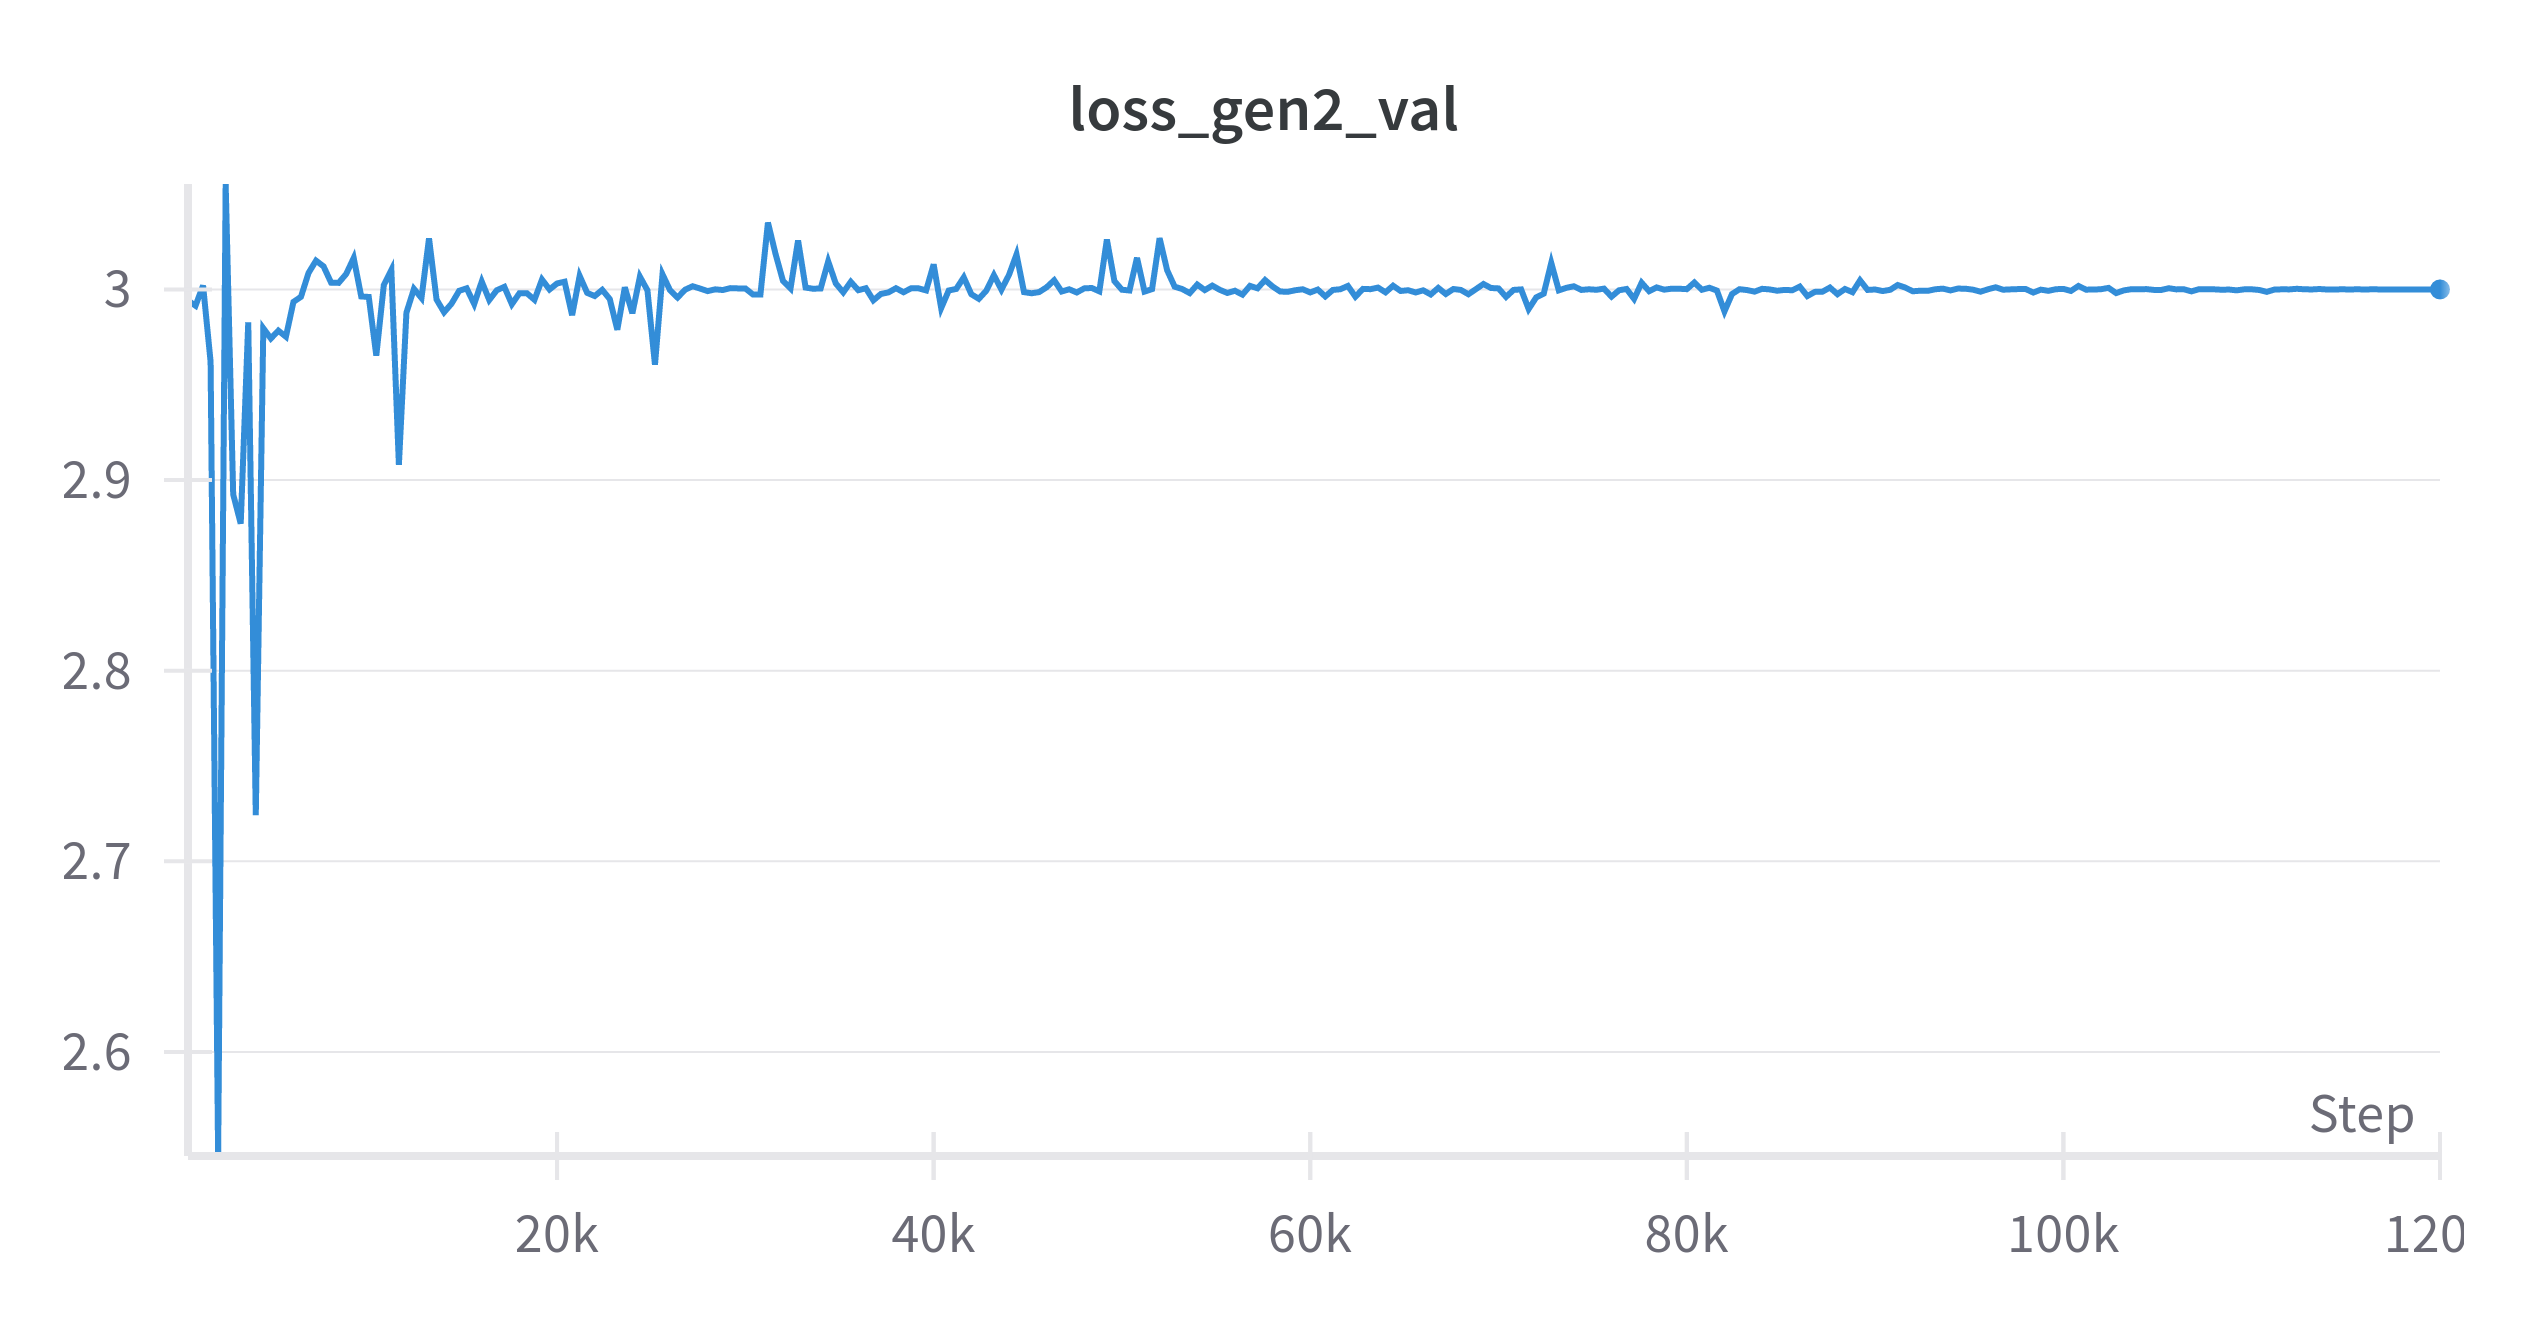
\includegraphics[width=0.4\textwidth]{loss-gen2-val.png} \\
    (c) & (d) \\
  \end{tabular}
  \caption{Generator Losses on Training and Validation Data}
  \label{tab:gen-losses}
\end{table}


\section{WAV synthesis samples, as desired}

\st{Unfortunately, this content is not available in your country}

Since the wavs cannot be reliably (cross-platformly) embedded into pdfs, they are available in the repo (check out the readme)


\clearpage

\section{Memes and fun content}

Since you were able to scroll that far, let me show you some fun content

\begin{figure}[htbp]
\centering

\includegraphics[width=0.8\textwidth]{meme-deadline-shift.jpg}

\label{fig:meme-deadline-shift}
\end{figure}

\begin{figure}[htbp]
\centering

\includegraphics[width=0.8\textwidth]{meme-stay-back.jpg}

\label{fig:meme-stay-back}
\end{figure}

\begin{figure}[htbp]
\centering
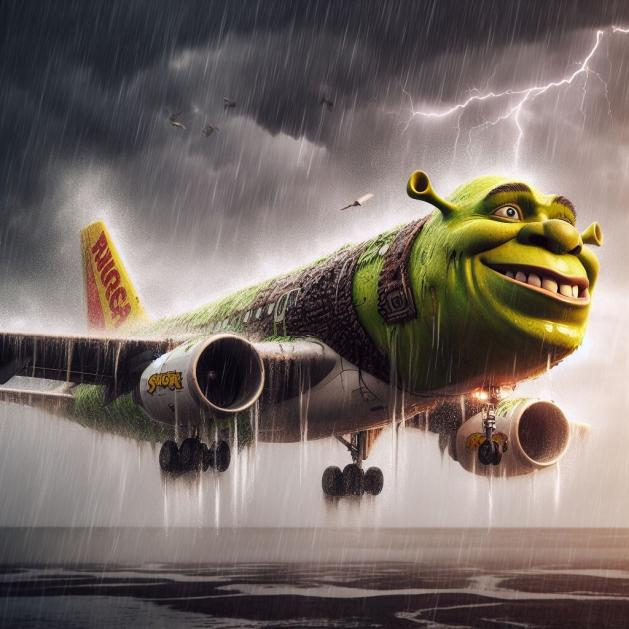
\includegraphics[width=0.8\textwidth]{meme-shrek-plane.jpg}

\label{fig:meme-shrek-plane}
\end{figure}

\begin{figure}[htbp]
\centering
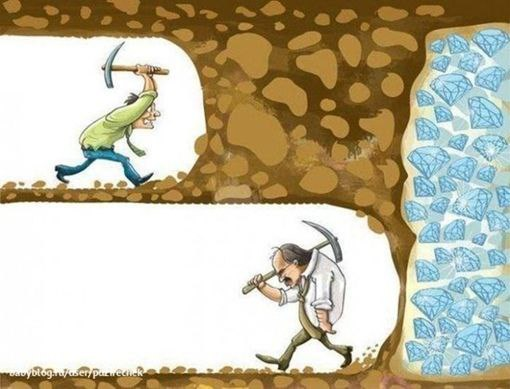
\includegraphics[width=0.8\textwidth]{meme-diamonds.jpg}

\label{fig:meme-diamonds}
\end{figure}

\begin{figure}[htbp]
\centering

\includegraphics[width=0.8\textwidth]{meme-brainwashed.jpg}

\label{fig:meme-brainwashed}
\end{figure}

\begin{figure}[htbp]
\centering

\includegraphics[width=0.8\textwidth]{meme-are-ya-winning.jpg}

\label{fig:meme-are-ya-winning}
\end{figure}

\begin{figure}[htbp]
\centering

\includegraphics[width=0.8\textwidth]{meme-cern-paper.png}

\label{fig:meme-cern-paper}
\end{figure}

\begin{figure}[htbp]
\centering

\includegraphics[width=0.8\textwidth]{meme-time-travel.jpg}

\label{fig:meme-time-travel}
\end{figure}

\begin{figure}[htbp]
\centering

\includegraphics[width=0.8\textwidth]{meme-conflicts.jpg}

\label{fig:meme-conflicts}
\end{figure}

\begin{figure}[htbp]
\centering
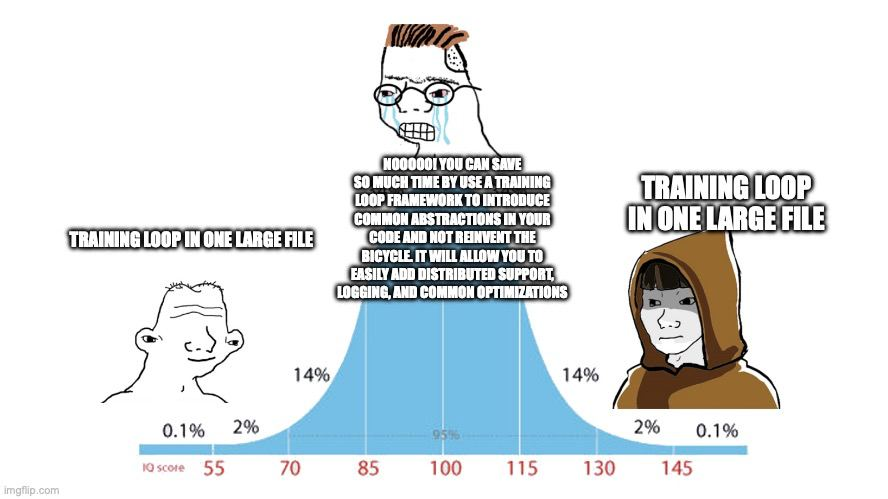
\includegraphics[width=0.8\textwidth]{meme-training-loop.jpg}

\label{fig:meme-training-loop}
\end{figure}

\begin{figure}[htbp]
\centering

\includegraphics[width=0.8\textwidth]{meme-fork.jpg}

\label{fig:meme-fork}
\end{figure}

\begin{figure}[htbp]
\centering

\includegraphics[width=0.8\textwidth]{meme-wrong-meme.jpg}

\label{fig:meme-wrong-meme}
\end{figure}

\begin{figure}[htbp]
\centering

\includegraphics[width=0.8\textwidth]{meme-transformer.png}

\label{fig:meme-transformer}
\end{figure}

\begin{figure}[htbp]
\centering

\includegraphics[width=0.8\textwidth]{meme-danger-genius.jpg}

\label{fig:meme-danger-genius}
\end{figure}

\begin{figure}[htbp]
\centering

\includegraphics[width=0.8\textwidth]{meme-problem.jpg}

\label{fig:meme-problem}
\end{figure}

\begin{figure}[htbp]
\centering

\includegraphics[width=0.8\textwidth]{meme-scam-banks.jpeg}

\label{fig:meme-scam-banks}
\end{figure}

\begin{figure}[htbp]
\centering
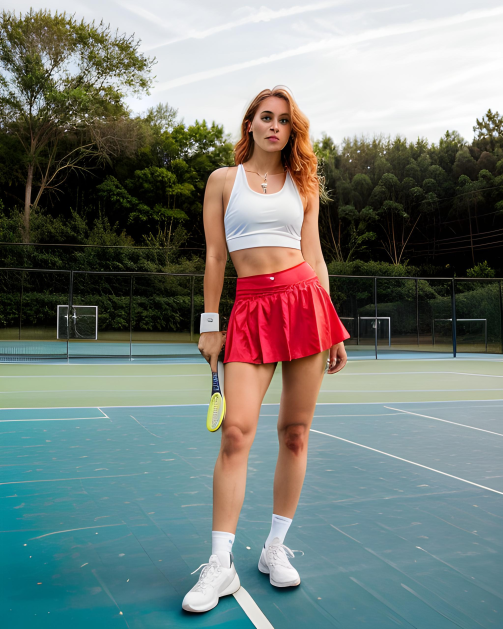
\includegraphics[width=0.8\textwidth]{meme-tennis.png}

\label{fig:meme-tennis}
\end{figure}

\begin{figure}[htbp]
\centering

\includegraphics[width=0.8\textwidth]{meme-time-to-go.png}

\label{fig:meme-time-to-go}
\end{figure}

\begin{figure}[htbp]
\centering
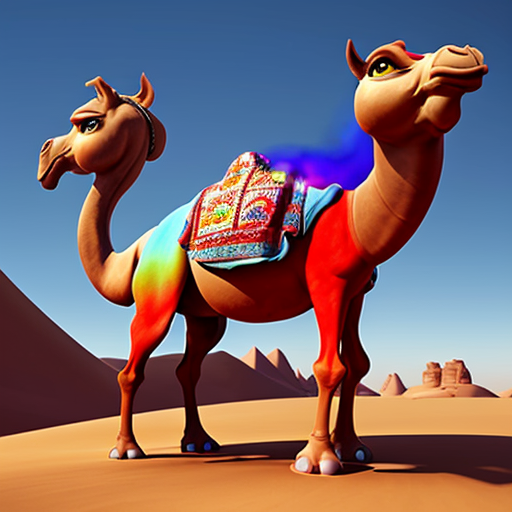
\includegraphics[width=0.8\textwidth]{meme-two-headed-camel.png}

\label{fig:meme-two-headed-camel}
\end{figure}

\clearpage

\begin{figure}[htbp]
\centering
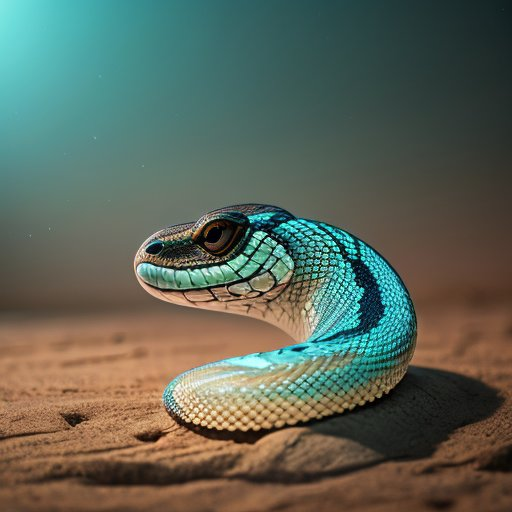
\includegraphics[width=0.8\textwidth]{meme-half-snake.jpg}

\label{fig:meme-half-snake}
\end{figure}

\begin{figure}[htbp]
\centering

\includegraphics[width=0.8\textwidth]{meme-delete-branch.jpg}

\label{fig:meme-delete-branch}
\end{figure}

\begin{figure}[htbp]
\centering

\includegraphics[width=0.8\textwidth]{meme-horseriders.png}

\label{fig:meme-horseriders}
\end{figure}

\begin{figure}[htbp]
\centering
\includegraphics[width=0.8\textwidth]{meme-cloudy-clouds.jpg}

\label{fig:meme-cloudy-clouds}
\end{figure}

\begin{figure}[htbp]
\centering
\includegraphics[width=0.8\textwidth]{meme-spam-drink.jpg}

\label{fig:meme-spam-drink}
\end{figure}

\begin{figure}[htbp]
\centering
\includegraphics[width=0.8\textwidth]{meme-good-design.jpg}

\label{fig:meme-good-design}
\end{figure}

\begin{figure}[htbp]
\centering
\includegraphics[width=0.8\textwidth]{meme-finally-won.jpeg}

\label{fig:meme-finally-won}
\end{figure}



\end{document}
